%Template Laporan PI
%Departemen Teknik Elektro dan Informatika
%Sekolah Vokasi UGM

%Dikembangkan oleh Dr. Fahmizal, S.T., M.Sc. dan Tim

%Perangkat lunak yang digunakan untuk mengolah LaTEX pada template ini adalah
%- TeXstudio
%- MiKTex
%- Overleaf (LaTEX editor berbasis daring)



\documentclass[12pt, a4paper, onecolumn, oneside, final]{report}

%Isi identitas proyek akhir disini

\providecommand{\judulid}{Judul Praktik Industri} 

\providecommand{\tempat}{(Nama Perusahaan)} %Nama Perusahaan KP
\providecommand{\place}{company name} % Company Name 
\providecommand{\penempatan}{Penempatan di perusahaan} %Penempatan lengkap di perusahaan

\providecommand{\penulis}{Nama Lengkap} %Nama Lengkap Mahasiswa 
\providecommand{\nim}{XX/XXXXXX/SV/XXXXX} % NIM

\providecommand{\tglMulai}{Hari/Bulan/Tahun} %Tanggal mulai KP
\providecommand{\tglSelesai}{Hari/Bulan/Tahun} %Tanggal selesai KP

\providecommand{\tipe}{Laporan Praktik Industri} %Tipe Laporan
\providecommand{\type}{Final Project} %Tipe Laporan
\providecommand{\prodi}{Teknologi Rekayasa Elektro} %Nama Prodi
\providecommand{\departemen}{Departemen Teknik Elektro dan Informatika}
\providecommand{\fakultas}{Sekolah Vokasi} %Nama Fakultas
\providecommand{\universitas}{Universitas Gadjah Mada} %Nama Universitas
\providecommand{\tglpengesahan}{\today} %Tanggal di Halaman Pengesahan
\providecommand{\tglpersetujuan}{\today} %Tanggal di Lembar Persetujuan
\providecommand{\tglpernyataan}{\today} %Tanggal di Surat Pernyataan

\providecommand{\tahun}{\the\year{}} %Tahun Proyek Akhir

\providecommand{\ketuapenguji}{Nama Ketua Penguji} %Nama Ketua Penguji
\providecommand{\NIPketuapenguji}{} %NIP Ketua Penguji

\providecommand{\sekretarispenguji}{Nama Sekretaris Penguji} %Nama Sekretaris Penguji
\providecommand{\NIPsekretarispenguji}{} %NIP Sekretaris Penguji

\providecommand{\anggotapenguji}{Nama Anggota Penguji} %Nama Anggota Penguji
\providecommand{\NIPanggotapenguji}{} %NIP Anggota Penguji

\providecommand{\dekan}{Nama Dekan.} %Nama Dekan
\providecommand{\NIPdekan}{} %NIP Dekan

\providecommand{\koordepartemen}{Nama koordepartemen} %Nama Koordepartemen
\providecommand{\NIPkoordepartemen}{} %NIP Koordepartemen

\providecommand{\koorprodi}{Nama Kaprodi} %Nama Kaprodi
\providecommand{\NIPkoorprodi}{} %NIP Kaprodi

\providecommand{\pembimbing}{Nama Dosen Pembimbing} %Nama Dosen Pembimbing
\providecommand{\NIPpembimbing}{} %NIP Dosen Pembimbing

\providecommand{\pimpinanPerusahaan}{Nama Lengkap dan gelar} %Nama Lengkap Pimpinan Perusahaan
\providecommand{\jabatanPimpinan}{Jabatan} %Jabatan Pimpinan Perusahaan

\providecommand{\pembimbingPerusahaan}{Nama Lengkap dan gelar} %Nama Pembimbing KP
\providecommand{\jabatanPembimbing}{Jabatan} %Jabatan Pembimbing KP

\providecommand{\katakunci}{kata kunci 1, kata kunci 2, kata kunci 2} %Kata kunci dalam Bahasa Indonesia
\providecommand{\keywords}{keyword 1, keyword 2, keyword 3} %Kata kunci dalam Bahasa Inggris

%\usepackage{caption}
%\usepackage{subcaption}

%memasukan PDF
\usepackage{pdfpages}

%\usepackage{multido}
%\usepackage{ifxetex}
%
%\ifxetex
%\newcount\pdflastximagepages
%\def\pdfximage#1{\pdflastximagepages=\XeTeXpdfpagecount"#1"\relax}
%\fi
%
%\def\filename{pst-fun-doc.pdf}
%\def\scale{0.4}
%\pdfximage{\filename}

% Diagram tikz
\usepackage{tikz-cd}

% Color
\usepackage{color}

% Mengatur bahasa latex
\usepackage[indonesian]{babel}
\usepackage[utf8]{inputenc}

% Untuk pengaturan spacing
\usepackage{setspace}
\onehalfspacing

% Untuk mengatur level section 
\setcounter{secnumdepth}{6}

% Digunakan untuk memasukan gambar ke laporan. 
\usepackage{graphicx}
\graphicspath{{gambar/}}
\usepackage{float}
\usepackage[hang,centerlast, nooneline ,small,md]{subfigure}
\usepackage[subfigure]{tocloft}

% Untuk mengatur spacing antara paragraf
\usepackage{parskip}

% Membuat indent
\usepackage{indentfirst}
\setlength\parindent{1cm}

% Untuk mengkustomisasi margin
\usepackage{scrextend}

% Untuk mengatur header dan footer
\usepackage{fancyhdr}

% Membuat seluruh tulisan menjadi Times New Roman. 
% \usepackage{pslatex}

% Merubah numbering chapter dan section untuk judul setiap bab menggunakan romawi dan judul anak bab menggunakan arabic
\renewcommand{\thesection}{\arabic{chapter}.\arabic{section}\hspace{0.05cm}}
\renewcommand{\thesubsection}{\arabic{chapter}.\arabic{section}.\arabic{subsection}\hspace{-0.25cm}}
\renewcommand{\thesubsubsection}{\Alph{subsubsection}.\hspace{-0,25cm}}
\renewcommand{\theparagraph}{\arabic{paragraph}.\hspace{-0,25cm}}

% Mengatur identasi judul section dan subsection
%\titleformat{\section}[block]{\bfseries}{\thesection.}{1em}{}
%\titleformat{\subsection}[block]{\hspace{2em}}{\thesubsection}{1em}{}

% Merubah huruf kapital pada judul daftar isi, daftar gambar, dan daftar table
\usepackage{tocloft}
\renewcommand{\cfttoctitlefont}{\hfil\large\bfseries\MakeUppercase}
\renewcommand{\cftloftitlefont}{\hfil\large\bfseries\MakeUppercase}
\renewcommand{\cftlottitlefont}{\hfil\large\bfseries\MakeUppercase}

\renewcommand\cftchappresnum{BAB }
\renewcommand\cftchapaftersnum{}
\newlength\mylen
\settowidth\mylen{\bfseries BAB 1 :\ } % if more than 9 chapters, use "Chapter 10"
\cftsetindents{chap}{0pt}{\mylen}

% Mengatur font section
\usepackage{sectsty}
\sectionfont{\fontsize{12}{14}\selectfont}
\subsectionfont{\fontsize{12}{14}\selectfont}
\subsubsectionfont{\fontsize{12}{14}\selectfont}
\paragraphfont{\normalfont\fontsize{12}{14}\selectfont}

% Untuk merupakan format penulisan BAB
\usepackage{titlesec}
%\titleformat*{\paragraph}{\normalfont\fontsize{12}{14}\selectfont}

\titleformat{\chapter}
{\doublespacing\fontsize{14pt}{16pt}\bfseries}
{\MakeUppercase{\chaptertitlename\ \Roman{chapter}}\filcenter}
{0.15cm}{\centering\uppercase}
\titlespacing*{\chapter}{0pt}{-1cm}{20pt}

% Mengatur spacing section
\titlespacing*{\section}
{0pt}{10pt}{0cm}
\titlespacing*{\subsection}
{0pt}{10pt}{0cm}
\titlespacing*{\subsubsection}
{0pt}{10pt}{0cm}
\titlespacing*{\paragraph}
{0pt}{10pt}{0cm}

% Digunakan untuk mengatur caption dalam dokumen.
\usepackage[font=footnotesize,format=plain,labelfont=bf,up,textfont=up]{caption}

% Untuk menghapus titik dua (colon)
\captionsetup[figure]{labelsep=space}
\captionsetup[table]{labelsep=space}

% Mengatur nomor caption gambar
\renewcommand{\thefigure}{\arabic{chapter}.\arabic{figure}}

% Mengatur nomor caption table
\renewcommand{\thetable}{\arabic{chapter}.\arabic{table}}

% Mengatur Hyphenation pada latex
\tolerance=1
\emergencystretch=\maxdimen
\hyphenpenalty=10000
\hbadness=10000

% Untuk mengatur setting indent
\setlength\parindent{1cm}

% Untuk memasukkan table
\usepackage{tabularx}
\usepackage{multirow}

% Untuk mengatur width
\usepackage{changepage}

% Menggatur setting halaman 
\usepackage{geometry}
\geometry{
    left=3cm,            % <-- you want to adjust this
    top=3cm,
    right=2.5cm,
    bottom=3cm,
}

% Teks testing
\usepackage{blindtext}
\usepackage{lipsum}

% Untuk mengatur subscript supscript
\usepackage{fixltx2e}

% Untuk formatting quote pada halaman motto
\usepackage{epigraph}

% Untuk mengatur wrap picture
\usepackage{wrapfig}

% Untuk notasi matematika
\usepackage{amsmath}
\usepackage{stmaryrd}
\usepackage{mathtools}



% untuk mengatur label nomor pada rumus
\renewcommand{\theequation}{\arabic{chapter}.\arabic{equation}}

% Untuk mengatur spacing daftar gambar
\newcommand*{\noaddvspace}{\renewcommand*{\addvspace}[1]{}}
\addtocontents{lof}{\protect\noaddvspace}

%Menambahkan sumber gambar
\usepackage{url}
\newcommand*{\putsource}[1]{%
	\textbf{\small{Sumber: }} \small{\url{#1}}
}

%untuk mengatur package include table in excel
% \usepackage{pgfplotstable}

% untuk mengatur landscape page
\usepackage{rotating}

%untuk mengubah page menjadi landscape
\usepackage{pdflscape}

% untuk list
\usepackage{enumitem}
\newenvironment{packed_enum}{
    \begin{enumerate}[leftmargin=1.5\parindent]
        \setlength{\itemsep}{0pt}
        \setlength{\parskip}{0pt}
        \setlength{\parsep}{0pt}
        }{\end{enumerate}}

\newenvironment{packed_item}{
    \begin{itemize}[leftmargin=1.5\parindent]
        \setlength{\itemsep}{0pt}
        \setlength{\parskip}{0pt}
        \setlength{\parsep}{0pt}
        }{\end{itemize}}

%paket untuk bibTex
\usepackage{cite}
\bibliographystyle{IEEEtran}
%\bibliographystyle{apalike}

%paket untuk mengembed kode dalam LaTeX
\usepackage{listings}
\lstset{
    basicstyle=\small,
    %basicstyle=\ttfamily,
    columns=fullflexible,
    frame=single,
}

%paket untuk tabel
\usepackage{longtable}
\usepackage[table,xcdraw]{xcolor}
\usepackage{tabularx}
\usepackage{multirow}

%paket untuk url
\usepackage{varioref}
% \usepackage{hyperref}
\usepackage[hidelinks]{hyperref} %remove red boxes
\usepackage{cleveref}

% styling python
\usepackage{color}
\usepackage{listings}    
\usepackage{courier}

\definecolor{mygreen}{rgb}{0,0.6,0}
\definecolor{mygray}{rgb}{0.5,0.5,0.5}
\definecolor{mymauve}{rgb}{0.58,0,0.82}

\lstset{ %
  backgroundcolor=\color{white},   % choose the background color
  basicstyle=\footnotesize,        % size of fonts used for the code
  breaklines=true,                 % automatic line breaking only at whitespace
  captionpos=b,                    % sets the caption-position to bottom
  commentstyle=\color{mygreen},    % comment style
  escapeinside={\%*}{*)},          % if you want to add LaTeX within your code
  keywordstyle=\color{blue},       % keyword style
  stringstyle=\color{mymauve},     % string literal style
}

%styling Processing
\usepackage{verbatim}

%Define Colors
\definecolor{black}{RGB}{0,0,0}
\definecolor{gray}{RGB}{102,102,102}		%#666666
\definecolor{function}{RGB}{0,102,153}		%#006699 lightblue
\definecolor{lightgreen}{RGB}{102,153,0}	%#669900
\definecolor{bluegreen}{RGB}{51,153,126}	%#33997e
\definecolor{magenta}{RGB}{217,74,122}	%#d94a7a
\definecolor{orange}{RGB}{226,102,26}		%#e2661a
\definecolor{purple}{RGB}{125,71,147}		%#7d4793
\definecolor{green}{RGB}{113,138,98}		%#718a62

\lstdefinelanguage{Processing}{
	%keyword1&2&6
	morekeywords = [3]{abstract, break, class, continue, default, enum, extends, false, final, finally, implements, import, instanceof, interface, native, new, null, package, private, protected, public, static, strictfp, throws, transient, true, void, volatile, length, assert, case, return, super, this, throw},
	%keyword3
	morekeywords = [4]{catch, do, for, if, else, switch, synchronized, while, try},
	%keyword4
	morekeywords = [5]{width, height, pixelHeight, displayHeight, displayWidth, focused, frameCount, frameRate, key, keyCode, keyPressed, mouseButton, mousePressed, mouseX, mouseY, pixels, pixelWidth, pmouseX, pmouseY},
	%keyword5
	morekeywords = [6]{Array, ArrayList, Boolean, Byte, BufferedReader, Character, Class, Double, Float, Integer, HashMap, PrintWriter, String, StringBuffer, StringBuilder, Thread, boolean, byte, char, color, double, float, int, long, short, FloatDict, FloatList, IntDict, IntList, JSONArray, JSONObject, PFont, PGraphics, PImage, PShader, PShape, PVector, StringDict, StringList, Table, TableRow, XML},
	%literal2
	morekeywords = [7]{ADD, ALIGN_CENTER, ALIGN_LEFT, ALIGN_RIGHT, ALPHA, ALPHA_MASK, ALT, AMBIENT, ARC, ARROW, ARGB, BACKSPACE, BASELINE, BEVEL, BLEND, BLUE_MASK, BLUR, BOTTOM, BOX, BURN, CENTER, CHATTER, CHORD, CLAMP, CLICK, CLOSE, CMYK, CODED, COMPLAINT, COMPOSITE, COMPONENT, CONCAVE_POLYGON, CONTROL, CONVEX_POLYGON, CORNER, CORNERS, CROSS, CUSTOM, DARKEST, DEGREES, DEG_TO_RAD, DELETE, DIAMETER, DIFFERENCE, DIFFUSE, DILATE, DIRECTIONAL, DISABLE_ACCURATE_2D, DISABLE_DEPTH_MASK, DISABLE_DEPTH_SORT, DISABLE_DEPTH_TEST, DISABLE_NATIVE_FONTS, DISABLE_OPENGL_ERRORS, DISABLE_PURE_STROKE, DISABLE_TEXTURE_MIPMAPS, DISABLE_TRANSFORM_CACHE, DISABLE_STROKE_PERSPECTIVE, DISABLED, DODGE, DOWN, DRAG, DXF, ELLIPSE, ENABLE_ACCURATE_2D, ENABLE_DEPTH_MASK, ENABLE_DEPTH_SORT, ENABLE_DEPTH_TEST, ENABLE_NATIVE_FONTS, ENABLE_OPENGL_ERRORS, ENABLE_PURE_STROKE, ENABLE_TEXTURE_MIPMAPS, ENABLE_TRANSFORM_CACHE, ENABLE_STROKE_PERSPECTIVE, ENTER, EPSILON, ERODE, ESC, EXCLUSION, EXIT, FX2D, GIF, GRAY, GREEN_MASK, GROUP, HALF, HALF_PI, HAND, HARD_LIGHT, HINT_COUNT, HSB, IMAGE, INVERT, JAVA2D, JPEG, LEFT, LIGHTEST, LINE, LINES, LINUX, MACOSX, MAX_FLOAT, MAX_INT, MIN_FOAT, MIN_INT, MITER, MODEL, MOVE, MULTIPLY, NORMAL, NORMALIZED, NO_DEPTH_TEST, NTSC, ONE, OPAQUE, OPEN, ORTHOGRAPHIC, OVERLAY, PAL, PDF, P2D, P3D, PERSPECTIVE, PI, PIE, PIXEL_CENTER, POINT, POINTS, POSTERIZE, PRESS, PROBLEM, PROJECT, QUAD, QUAD_STRIP, QUADS, QUARTER_PI, RAD_TO_DEG, RADIUS, RADIANS, RECT, RED_MASK, RELEASE, REPEAT, REPLACE, RETURN, RGB, RIGHT, ROUND, SCREEN, SECAM, SHAPE, SHIFT, SPAN, SPECULAR, SPHERE, SOFT_LIGHT, SQUARE, SUBTRACT, SVG, SVIDEO, TAB, TARGA, TAU, TEXT, TFF, THIRD_PI, THRESHOLD, TIFF, TOP, TRIANGLE, TRIANGLE_FAN, TRIANGLES, TRIANGLE_STRIP, TUNER, TWO, TWO_PI, UP, WAIT, WHITESPACE},
	%function1
	morekeywords = [8]{start, stop, breakShape, createPath, loadMatrix, parseBoolean, parseByte, parseChar, parseFloat, parseInt, saveFile, savePath, sketchFile, sketchPath, abs, acos, alpha, ambient, ambientLight, append, applyMatrix, arc, arrayCopy, asin, atan, atan2, background, beginCamera, beginContour, beginRaw, beginRecord, beginShape, bezier, bezierDetail, bezierPoint, bezierTangent, bezierVertex, binary, blend, blendColor, blendMode, blue, box, brightness, camera, ceil, circle, clear, clip, color, colorMode, concat, constrain, copy, cos, createFont, createGraphics, createImage, createInput, createOutput, createReader, createShape, createWriter, cursor, curve, curveDetail, curvePoint, curveTangent, curveTightness, curveVertex, day, degrees, delay, directionalLight, displayDensity, dist, ellipse, ellipseMode, emissive, endCamera, endContour, endRaw, endRecord, endShape, exit, exp, expand, fill, filter, floor, frustum, fullScreen, get, green, hex, hint, hour, hue, image, imageMode, join, launch, lerp, lerpColor, lightFalloff, lights, lightSpecular, line, loadBytes, loadFont, loadImage, loadJSONArray, loadJSONObject, loadPixels, loadShader, loadShape, loadStrings, loadTable, loadXML, log, loop, mag, map, match, matchAll, max, millis, min, minute, modelX, modelY, modelZ, month, nf, nfc, nfp, nfs, noClip, noCursor, noFill, noise, noiseDetail, noiseSeed, noLights, noLoop, norm, normal, noSmooth, noStroke, noTint, ortho, parseJSONArray, parseJSONObject, parseXML, perspective, list, pixelDensity, point, pointLight, popMatrix, popStyle, pow, print, printArray, printCamera, println, printMatrix, printProjection, pushMatrix, pushStyle, quad, quadraticVertex, radians, random, randomGaussian, randomSeed, rect, rectMode, red, redraw, requestImage, resetMatrix, resetShader, reverse, rotate, rotateX, rotateY, rotateZ, round, saturation, save, saveBytes, saveFrame, saveJSONArray, saveJSONObject, saveStream, saveStrings, saveTable, saveXML, scale, screenX, screenY, screenZ, second, selectFolder, selectInput, selectOutput, set, shader, shape, shapeMode, shearX, shearY, shininess, shorten, sin, size, smooth, sort, specular, sphere, sphereDetail, splice, split, splitTokens, spotLight, sq, sqrt, square, stroke, strokeCap, strokeJoin, strokeWeight, subset, tan, text, textAlign, textAscent, textDescent, textFont, textLeading, textMode, textSize, texture, textureMode, textureWrap, textWidth, thread, tint, translate, triangle, trim, unbinary, unhex, updatePixels, vertex, year},
	%function2
	morekeywords = [9]{cache, readLine, close, flush, print, println, charAt, equals, indexOf, substring, toLowerCase, toUpperCase, getDouble, getLong, getColumnTitles, getColumnTypes, getColumnType, setDouble, setLong, add, clear, div, get, hasKey, keyArray, keys, mult, remove, set, size, sortKeys, sortKeysReverse, sortValues, sortValuesReverse, sub, valueArray, values, append, array, hasValue, max, min, mult, remove, reverse, shuffle, sort, sortReverse, increment, getBoolean, getFloat, getInt, getIntArray, getJSONArray, getJSONObject, getString, getStringArray, isNull, setBoolean, setFloat, setInt, setJSONArray, setJSONObject, setString, beginDraw, endDraw, blend, copy, filter, loadPixels, mask, resize, save, updatePixels, addChild, beginContour, beginShape, disableStyle, enableStyle, endContour, endShape, getChild, getChildCount, getVertex, getVertexCount, isVisible, resetMatrix, rotate, rotateX, rotateY, rotateZ, scale, setFill, setStroke, setVertex, setVisible, translate, angleBetween, cross, dist, dot, fromAngle, heading, lerp, limit, mag, magSq, normalize, random2D, random3D, setMag, lower, upper, addColumn, addRow, clearRows, findRow, findRows, getColumnCount, getRow, getRowCount, getStringColumn, matchRow, matchRows, removeColumn, removeRow, removeTokens, rows, trim, getColumnTitle, format, getAttributeCount, getChildren, getContent, getName, getParent, hasAttribute, hasChildren, listAttributes, listChildren, removeChild, setContent, setName, toString},
	%function4
	morekeywords = [10]{draw, keyReleased, keyTyped, mouseClicked, mouseDragged, mouseMoved, mouseReleased, mouseWheel, settings, setup},
	keywordstyle = [3]\color{bluegreen},
	keywordstyle = [4]\color{lightgreen},
	keywordstyle = [5]\color{magenta},
	keywordstyle = [6]\color{orange},
	keywordstyle = [7]\color{green},
	keywordstyle = [8]\color{function},
	keywordstyle = [9]\color{function},
	keywordstyle = [10]\color{function}\bfseries,
	sensitive = true,
	morecomment = [l][\color{gray}]{//},
	morecomment = [s][\color{gray}]{/*}{*/},
	morecomment = [s][\color{gray}]{/**}{*/},
	morestring = [b][\color{purple}]",
	morestring = [b][\color{purple}]'
}
\renewcommand{\ttdefault}{pcr}
\lstset{
	language={Processing},
	basicstyle={\small\ttfamily},
	identifierstyle={\small},
	commentstyle={\small\itshape},
	keywordstyle={\small},
	ndkeywordstyle={\small},
	stringstyle={\small\ttfamily},
	frame={tb},
	breaklines=true,
	columns=[l]{fullflexible},
	numbers=left,
	xrightmargin=0em,
	xleftmargin=3em,
	numberstyle={\scriptsize},
	stepnumber=1,
	numbersep=1em,
	lineskip=-0.5ex,
}

%listing style

\definecolor{codegreen}{rgb}{0,0.6,0}
\definecolor{codegray}{rgb}{0.5,0.5,0.5}
\definecolor{codepurple}{rgb}{0.58,0,0.82}
\definecolor{backcolour}{rgb}{0.95,0.95,0.92}

\lstdefinestyle{custom}{
	frame = single,
	backgroundcolor=\color{backcolour},   
	commentstyle=\color{codegreen},
	keywordstyle=\color{magenta},
	numberstyle=\tiny\color{codegray},
	stringstyle=\color{codepurple},
	basicstyle=\ttfamily\footnotesize,
	breakatwhitespace=false,         
	breaklines=true,                 
	captionpos=b,                    
	keepspaces=true,                 
	numbers=left,                    
	numbersep=6pt,                  
	showspaces=false,                
	showstringspaces=false,
	showtabs=false,                  
	tabsize=2
}

\lstset{style=custom}

\usepackage{amssymb}




\hyphenation{di-la-ku-kan} %bisa dilihat di bagian "abstrak"

%tulis seperlunya, kalau menemukan kata yang terpenggal salah, misalnya.. 
\hyphenation{be-ri-kut}
\hyphenation{a-da-lah} %dsb.. 

\begin{document}
\begin{titlepage}
    \begin{center}
        \begin{doublespace}
            \textbf{\MakeUppercase{\large{\tipe}}}\\[0.5cm]
            \textbf{\MakeUppercase{\normalsize{\judulid}}}\\
            \textbf{\MakeUppercase{\normalsize{\tempat}}}\\[2.5cm]
            
%            \textbf{\MakeUppercase{\large{\judulen}}}\\[1cm]
        \end{doublespace}
        
\includegraphics[width=0.35\linewidth]{gambar/logo-ugm.png}\\[1cm]

        \textbf{\normalsize {Oleh:}} \\
        \textbf{\normalsize \MakeUppercase{\underline{\penulis}}} \\
        \textbf{\normalsize \MakeUppercase{{\nim}}} \\[4cm]


        \textbf{\normalsize \MakeUppercase{Program Studi Sarjana Terapan \\ \prodi}}\\
        \textbf{\normalsize \MakeUppercase{\departemen}}\\
        \textbf{\normalsize \MakeUppercase{\fakultas}}\\
        \textbf{\normalsize \MakeUppercase{\universitas}}\\
        \textbf{\normalsize \the\year{}}\\
    \end{center}
\end{titlepage}
\pagenumbering{roman}
\begin{titlepage}
    \begin{center}

        \begin{doublespace}
            \textbf{\MakeUppercase{\large{\tipe}}}\\[0.5cm]\textbf{\MakeUppercase{\normalsize{\judulid}}}\\[3cm]
            
%            \textbf{\MakeUppercase{\large{\judulen}}}\\[1cm]
        \end{doublespace}
        {\tipe}\\
        Program Studi {\prodi} \\[2cm]
        Diajukan untuk memenuhi salah satu syarat memperoleh gelar Sarjana Terapan Teknik pada Program Studi {\prodi} {\departemen} {\fakultas} {\universitas}\\[3cm]
        
%        
\includegraphics[width=0.35\linewidth]{gambar/logo-ugm.png}\\[1cm]

        \textbf{\normalsize {Oleh:}} \\
        \textbf{\normalsize \MakeUppercase{\underline{\penulis}}} \\
        \textbf{\normalsize \MakeUppercase{{\nim}}} \\[3cm]


        \textbf{\normalsize \MakeUppercase{Program Studi Sarjana Terapan\\ \prodi}}\\
        \textbf{\normalsize \MakeUppercase{\departemen}}\\
        \textbf{\normalsize \MakeUppercase{\fakultas}}\\
        \textbf{\normalsize \MakeUppercase{\universitas}}\\
        \textbf{\normalsize \the\year{}}\\
    \end{center}
\end{titlepage}
%lembar pengesahan
\newpage
%\thispagestyle{empty}
\addcontentsline{toc}{chapter}{HALAMAN PENGESAHAN}

\begin{tikzpicture}[remember picture, overlay]
	\node at (current page.center) {
\includegraphics[height=10cm]{gambar/logo-ugm-emas.jpeg}};
\end{tikzpicture}

\begin{center}
    \begin{doublespace}
        \textbf{\large \MakeUppercase{HALAMAN PENGESAHAN\\ PRAKTIK INDUSTRI}}
    \end{doublespace}
\end{center}

\begin{center}
    %\textbf{\large \MakeUppercase {\judulid}}
        \textbf{\normalsize \MakeUppercase {\judulid}}
\end{center}

\begin{center}
    Disusun oleh:\\
    \textbf{\penulis}\\
    \textbf{\nim}\\[0.5cm]

    Diajukan untuk memenuhi salah satu syarat memperoleh gelar Sarjana Terapan Teknik pada Program Studi {\prodi} {\departemen} {\fakultas} {\universitas}\\[1cm]
\end{center}

\begin{center}
    \textbf{Hasil dari Praktik Industri ini telah diseminarkan pada:}
\end{center}

\begin{table}[h!]
    \begin{tabular}{p{1cm} p{3cm} p{1cm} l}
        & \textbf{Hari, Tanggal} & \textbf{:} & \\ 
        & \textbf{Pukul}         & \textbf{:} & \\ 
        & \textbf{Tempat}        & \textbf{:} & \\[1cm]
    \end{tabular}
    \label{tabel1}
\end{table}

\begin{center}
    Diterima dan disetujui oleh,
\end{center}

\begin{center}
    Mengetahui, \\[1cm]
\end{center}
\begin{minipage}{0.35\textwidth}
    Ketua Program Studi\\
    Teknologi Rekayasa Elektro\\[2.5cm]
    \underline{\koorprodi}\\
    NIP. \NIPkoorprodi
\end{minipage}%
\hfill
 \begin{minipage}{0.35\textwidth}
    Dosen Pembimbang \\
    Praktik Industri \\[2cm]
    
    \underline{\pembimbing}\\
    NIP. \NIPpembimbing
\end{minipage}
%lembar pengesahan
\newpage
%\thispagestyle{empty}
\addcontentsline{toc}{chapter}{HALAMAN PENGESAHAN}

\begin{center}
    \begin{doublespace}
        \textbf{\large \MakeUppercase{Halaman Pengesahan \\ Praktik Industri}}
    \end{doublespace}
\end{center}

\begin{center}
    \textbf{\normalsize \MakeUppercase {\judulid}} \\
    \textbf{\normalsize \MakeUppercase {\tempat}} \\ [5cm]
\end{center}

\begin{center}
    Disusun oleh:\\
    \textbf{\underline{\penulis}}\\
    \textbf{\nim}\\[4cm]

    Telah melaksanakan kegiatan Praktik Industri \\
    dari tanggal \textbf{\tglMulai} sampai dengan \textbf{\tglSelesai} \\ [2cm]
\end{center}

\begin{center}
    Mengetahui, \\[1cm]
\end{center}
\begin{minipage}{0.45\textwidth}
    Kepala/Pimpinan/Supervisor\\
    \tempat,\\[2cm]
    \underline{\pimpinanPerusahaan}\\
    \jabatanPimpinan
\end{minipage}%
\hfill
 \begin{minipage}{0.35\textwidth}
    Telah diperiksa dan disetujui \\
    Pembimbing Praktik Industri\\[2cm]
    \underline{\pembimbingPerusahaan}\\
    \jabatanPembimbing
\end{minipage}
\clearpage
\phantomsection
\addcontentsline{toc}{chapter}{KATA PENGANTAR}
\begin{center}
    \textbf{\large KATA PENGANTAR}\\[3em]
\end{center}
%-----------------------------------------

Puji syukur kehadirat Allah SWT atas berkat rahmat dan karunia-Nya, {\tipe} dalam rangka untuk memenuhi sebagian persyaratan untuk mendapatkan gelar Sarjana Terapan.

{\tipe} ini dapat diselesaikan tidak lepas dari bantuan dan kerjasama dari berbagai pihak. Berkenaan dengan hal tersebut, penulis menyampaikan ucapan terima kasih kepada yang terhormat:

\begin{enumerate}
    \item Ucapan terimakasih 1
    \item Ucapan terimakasih 2
    \item Ucapan terimakasih 3
    \item Ucapan terimakasih 4
    \item Ucapan terimakasih 5
\end{enumerate}

Akhirnya, semoga segala bantuan yang telah diberikan oleh semua pihak dapat menjadi amalan yang bermanfaat dan mendapatkan buah karma baik di masa kini maupun di masa mendatang. Semoga {\tipe} ini menjadi informasi bermanfaat bagi pembaca atau pihak lain yang membutuhkannya.

\begin{flushright}
    Yogyakarta, \tglpengesahan\\[1.25cm]
    {\underline{{\penulis}}} \\
    \nim
\end{flushright}
% Table of contents
\clearpage
\phantomsection
\addcontentsline{toc}{chapter}{DAFTAR ISI}
%\renewcommand{\cftdotsep}{\cftnodots}
\setlength{\cftbeforetoctitleskip}{-0.5cm}
\renewcommand{\cfttoctitlefont}{\hfill\large\bfseries}
\renewcommand{\cftaftertoctitle}{\hfill\hfill}
\renewcommand\contentsname{DAFTAR ISI}
\tableofcontents
% List of fig
\clearpage
\phantomsection
\addcontentsline{toc}{chapter}{DAFTAR GAMBAR}
\setlength{\cftbeforeloftitleskip}{-0.5cm}
\renewcommand{\cftloftitlefont}{\hfill\large\bfseries}
\renewcommand{\cftafterloftitle}{\hfill}
\renewcommand{\cftfigleader}{\dotfill}
\renewcommand\listfigurename{DAFTAR GAMBAR}
\listoffigures
% List of table
\clearpage
\phantomsection
\addcontentsline{toc}{chapter}{DAFTAR TABEL}
\setlength{\cftbeforeloftitleskip}{-0.5cm}
\renewcommand{\cftloftitlefont}{\hfill\large\bfseries}
\renewcommand{\cftafterloftitle}{\hfill}
\renewcommand{\cfttableader}{\dotfill}
\renewcommand\listtablename{\centerline {\large\bfseries  DAFTAR TABEL}}
\listoftables
\clearpage
\phantomsection
\addcontentsline{toc}{chapter}{DAFTAR SINGKATAN}

\begin{center}
    \large \textbf{DAFTAR SINGKATAN} \\
    {\normalsize (bila ada)}
\end{center}
\vspace{3em}

\begin{center}
    \begin{tabularx}{0.8\textwidth} {
            >{\raggedright\arraybackslash}X
            >{\raggedright\arraybackslash}X}
        \hline
        \textbf{Notasi} & \textbf{Arti}                    \\
        \hline
        PID     & \textit{\textit{proporsional, integral, derivatif}}\\
        $K_{p}$ & \textit{Proportional gain}\\
        $K_{i}$ & \textit{Integral gain}\\
        $K_{d}$ & \textit{Derivative gain}\\
        \hline
    \end{tabularx}
\end{center}
%\chapter{ABSTRAK}
\clearpage
\phantomsection
\addcontentsline{toc}{chapter}{INTISARI}
\begin{center}
   \textbf{\large{\judulid}}\\[0.5cm]
   Oleh :\\
   \penulis\\
   \nim\\[2em]
    \textbf{INTISARI}\\[0.5cm]
\end{center}

\lipsum[2-4]

\noindent Kata kunci: \katakunci
\include{chapters/daftarlampiran}

\pagenumbering{arabic}
\chapter[PENDAHULUAN]{\\ PENDAHULUAN}

\section{Latar Belakang}

\lipsum[1] ~\cite{chan2013review}

\section{Tujuan dan Manfaat}
Berikut adalah beberapa tujuan penelitian yang telah ditetapkan untuk memandu jalannya penelitian ini: 
\begin{enumerate}
    \item Tujuan Penelitian 1
    \item Tujuan Penelitian 2
    \item Tujuan Penelitian 3
\end{enumerate}

\section{Waktu dan Tempat Pelaksanaan}
\begin{table}[h!]
    \begin{tabular}{p{1cm} p{1.5cm} p{0.25cm} p{11.25cm}}
        & Waktu  & : & {\tglMulai} - {\tglSelesai} \\ 
        & Tempat & : & {\penempatan} \\
    \end{tabular}
    \label{tabel2}
\end{table}
\chapter[PROFIL PERUSAHAAN]{\\ PROFIL PERUSAHAAN}

\section{Sejarah Singkat Perusahaan}
\lipsum[1]

\section{Struktur Organisasi}
\lipsum[1]

\section{Tugas dan Tanggung Jawab}
\lipsum[1]

\begin{packed_enum}
    \item Tugas dan Tanggung Jawab 1
    \item Tugas dan Tanggung Jawab 2
    \item Tugas dan Tanggung Jawab 3
    \item Tugas dan Tanggung Jawab 4
\end{packed_enum}

\section{Kesehatan dan Keselamatan Kerja (K3)}
\lipsum[1]

\begin{table}[H]
    \centering
    \caption{Contoh Tabel 2}
    \label{t blok}
    \begin{tabular}{|c|l|l|}
        \hline
        \rowcolor[HTML]{C0C0C0} 
        {\color[HTML]{000000} No.} & \multicolumn{1}{c|}{\cellcolor[HTML]{C0C0C0}{\color[HTML]{000000} Nama}} & \multicolumn{1}{c|}{\cellcolor[HTML]{C0C0C0}Fungsi}  \\ \hline
        \rowcolor[HTML]{FFFFFF} 
        1 & \textit{Nama rincian objek yang akan dibahas 1} & Fungsi rincian objek penjelasan 1 \\ \hline
        2 & \textit{Nama rincian objek yang akan dibahas 2} & Fungsi rincian objek penjelasan 2 \\ \hline
        3 & \textit{Nama rincian objek yang akan dibahas 3} & Fungsi rincian objek penjelasan 3 \\ \hline
        4 & \textit{Nama rincian objek yang akan dibahas 4} & Fungsi rincian objek penjelasan 4 \\ \hline
    \end{tabular}
\end{table}

\section{Etika Profesi}
\lipsum[2]
\chapter[POKOK PEMBAHASAN]{\\ POKOK PEMBAHASAN}
\lipsum[1]

\section{Perangkat Penelitian}
\lipsum[1]

\section{Penjelasan Tahapan Penelitian 1}
\lipsum[1]

\subsection{Sub Penjelasan Tahapan Penelitian 1}
\lipsum[1]

\begin{figure}[H]
    \centering
    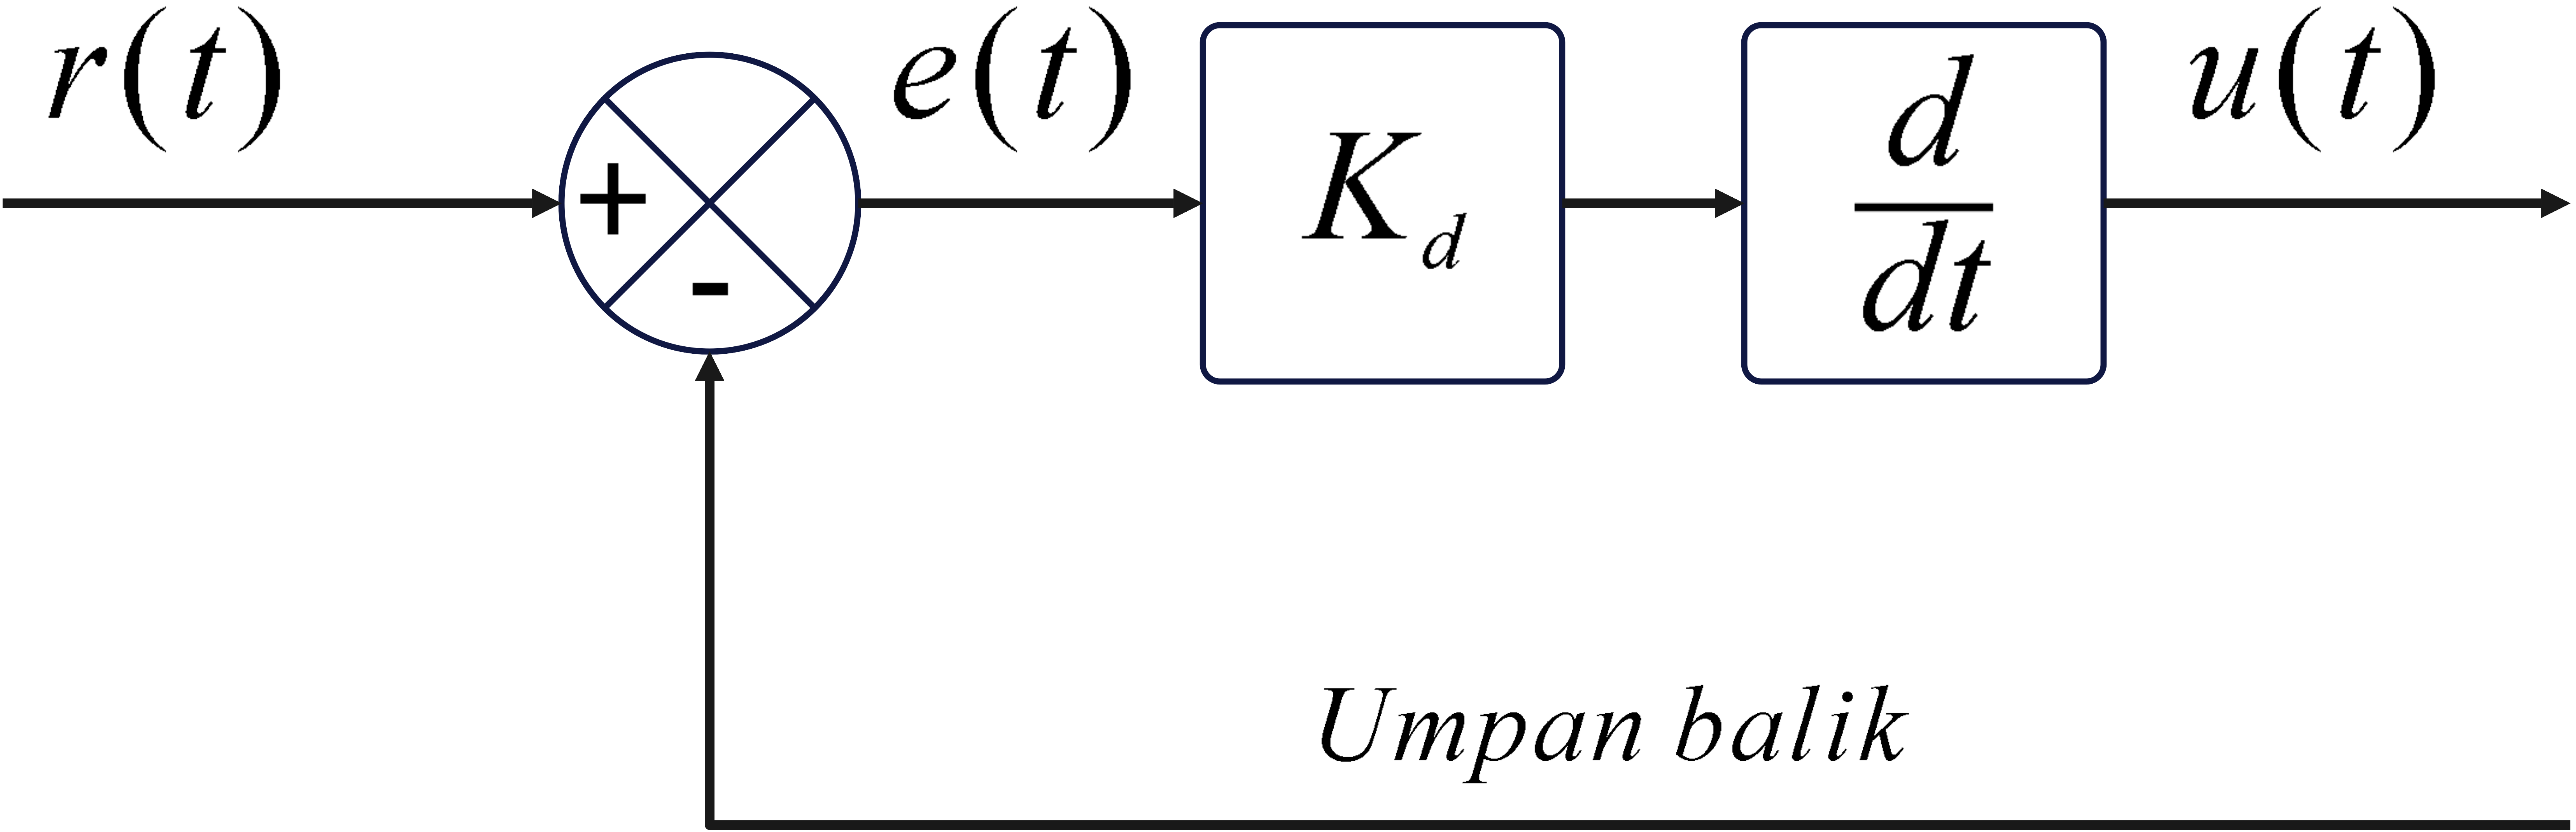
\includegraphics[width=0.8\linewidth]{gambar/diagram.png}
    \caption{Contoh gambar 1}
    \label{gambar1}
\end{figure}

\lipsum[1]

\subsection{Sub Penjelasan Tahapan Penelitian 1}
\lipsum[1]

\section{Penjelasan Tahapan Penelitian 2}
\lipsum[1]

\subsection{Sub Penjelasan Tahapan Penelitian 2}
\lipsum[1]

\begin{table}[H]
	\centering
	\caption{Contoh tabel 3}
	\label{t alpha}
	\begin{tabular}{|c|cccccccc|}
		\hline
		\rowcolor[HTML]{000000} 
		{\color[HTML]{333333} }                                                    & \multicolumn{8}{c|}{\cellcolor[HTML]{000000}{\color[HTML]{FFFFFF} $\dot{e}(k)$}} \\ \hline
		\rowcolor[HTML]{9B9B9B} 
		\cellcolor[HTML]{000000}{\color[HTML]{FFFFFF} }                            & \multicolumn{1}{c|}{\cellcolor[HTML]{9B9B9B}{\color[HTML]{333333} }}   & \multicolumn{1}{c|}{\cellcolor[HTML]{9B9B9B}{\color[HTML]{333333} NB}} & \multicolumn{1}{c|}{\cellcolor[HTML]{9B9B9B}{\color[HTML]{333333} NM}} & \multicolumn{1}{c|}{\cellcolor[HTML]{9B9B9B}{\color[HTML]{333333} NS}} & \multicolumn{1}{c|}{\cellcolor[HTML]{9B9B9B}{\color[HTML]{333333} ZO}} & \multicolumn{1}{c|}{\cellcolor[HTML]{9B9B9B}{\color[HTML]{333333} PS}} & \multicolumn{1}{c|}{\cellcolor[HTML]{9B9B9B}{\color[HTML]{333333} PM}} & {\color[HTML]{333333} PB} \\ \cline{2-9} 
		\rowcolor[HTML]{FFFFFF} 
		\cellcolor[HTML]{000000}{\color[HTML]{FFFFFF} }                            & \multicolumn{1}{c|}{\cellcolor[HTML]{9B9B9B}{\color[HTML]{333333} NB}} & \multicolumn{1}{c|}{\cellcolor[HTML]{FFFFFF}{\color[HTML]{333333} S}}  & \multicolumn{1}{c|}{\cellcolor[HTML]{FFFFFF}{\color[HTML]{333333} S}}  & \multicolumn{1}{c|}{\cellcolor[HTML]{FFFFFF}{\color[HTML]{333333} S}}  & \multicolumn{1}{c|}{\cellcolor[HTML]{FFFFFF}{\color[HTML]{333333} S}}  & \multicolumn{1}{c|}{\cellcolor[HTML]{FFFFFF}{\color[HTML]{333333} S}}  & \multicolumn{1}{c|}{\cellcolor[HTML]{FFFFFF}{\color[HTML]{333333} S}}  & {\color[HTML]{333333} S}  \\ \cline{2-9} 
		\rowcolor[HTML]{FFFFFF} 
		\cellcolor[HTML]{000000}{\color[HTML]{FFFFFF} }                            & \multicolumn{1}{c|}{\cellcolor[HTML]{9B9B9B}{\color[HTML]{333333} NM}} & \multicolumn{1}{c|}{\cellcolor[HTML]{FFFFFF}{\color[HTML]{333333} MS}}  & \multicolumn{1}{c|}{\cellcolor[HTML]{FFFFFF}{\color[HTML]{333333} MS}}  & \multicolumn{1}{c|}{\cellcolor[HTML]{FFFFFF}{\color[HTML]{333333} S}}  & \multicolumn{1}{c|}{\cellcolor[HTML]{FFFFFF}{\color[HTML]{333333} S}}  & \multicolumn{1}{c|}{\cellcolor[HTML]{FFFFFF}{\color[HTML]{333333} S}}  & \multicolumn{1}{c|}{\cellcolor[HTML]{FFFFFF}{\color[HTML]{333333} MS}}  & {\color[HTML]{333333} MS}  \\ \cline{2-9} 
		\rowcolor[HTML]{FFFFFF} 
		\cellcolor[HTML]{000000}{\color[HTML]{FFFFFF} }                            & \multicolumn{1}{c|}{\cellcolor[HTML]{9B9B9B}{\color[HTML]{333333} NS}} & \multicolumn{1}{c|}{\cellcolor[HTML]{FFFFFF}{\color[HTML]{333333} M}}  & \multicolumn{1}{c|}{\cellcolor[HTML]{FFFFFF}{\color[HTML]{333333} MS}}  & \multicolumn{1}{c|}{\cellcolor[HTML]{FFFFFF}{\color[HTML]{333333} MS}}  & \multicolumn{1}{c|}{\cellcolor[HTML]{FFFFFF}{\color[HTML]{333333} S}}  & \multicolumn{1}{c|}{\cellcolor[HTML]{FFFFFF}{\color[HTML]{333333} MS}}  & \multicolumn{1}{c|}{\cellcolor[HTML]{FFFFFF}{\color[HTML]{333333} MS}}  & {\color[HTML]{333333} M}  \\ \cline{2-9} 
		\rowcolor[HTML]{FFFFFF} 
		\cellcolor[HTML]{000000}{\color[HTML]{FFFFFF} }                            & \multicolumn{1}{c|}{\cellcolor[HTML]{9B9B9B}{\color[HTML]{333333} ZO}} & \multicolumn{1}{c|}{\cellcolor[HTML]{FFFFFF}{\color[HTML]{333333} B}}  & \multicolumn{1}{c|}{\cellcolor[HTML]{FFFFFF}{\color[HTML]{333333} M}}  & \multicolumn{1}{c|}{\cellcolor[HTML]{FFFFFF}{\color[HTML]{333333} MS}}  & \multicolumn{1}{c|}{\cellcolor[HTML]{FFFFFF}{\color[HTML]{333333} MS}}  & \multicolumn{1}{c|}{\cellcolor[HTML]{FFFFFF}{\color[HTML]{333333} MS}}  & \multicolumn{1}{c|}{\cellcolor[HTML]{FFFFFF}{\color[HTML]{333333} M}}  & {\color[HTML]{333333} B}  \\ \cline{2-9} 
		\rowcolor[HTML]{FFFFFF} 
		\cellcolor[HTML]{000000}{\color[HTML]{FFFFFF} }                            & \multicolumn{1}{c|}{\cellcolor[HTML]{9B9B9B}{\color[HTML]{333333} PS}} & \multicolumn{1}{c|}{\cellcolor[HTML]{FFFFFF}{\color[HTML]{333333} M}}  & \multicolumn{1}{c|}{\cellcolor[HTML]{FFFFFF}{\color[HTML]{333333} MS}}  & \multicolumn{1}{c|}{\cellcolor[HTML]{FFFFFF}{\color[HTML]{333333} MS}}  & \multicolumn{1}{c|}{\cellcolor[HTML]{FFFFFF}{\color[HTML]{333333} S}}  & \multicolumn{1}{c|}{\cellcolor[HTML]{FFFFFF}{\color[HTML]{333333} MS}}  & \multicolumn{1}{c|}{\cellcolor[HTML]{FFFFFF}{\color[HTML]{333333} MS}}  & {\color[HTML]{333333} M}  \\ \cline{2-9} 
		\rowcolor[HTML]{FFFFFF} 
		\cellcolor[HTML]{000000}{\color[HTML]{FFFFFF} }                            & \multicolumn{1}{c|}{\cellcolor[HTML]{9B9B9B}{\color[HTML]{333333} PM}} & \multicolumn{1}{c|}{\cellcolor[HTML]{FFFFFF}{\color[HTML]{333333} MS}}  & \multicolumn{1}{c|}{\cellcolor[HTML]{FFFFFF}{\color[HTML]{333333} MS}}  & \multicolumn{1}{c|}{\cellcolor[HTML]{FFFFFF}{\color[HTML]{333333} S}}  & \multicolumn{1}{c|}{\cellcolor[HTML]{FFFFFF}{\color[HTML]{333333} S}}  & \multicolumn{1}{c|}{\cellcolor[HTML]{FFFFFF}{\color[HTML]{333333} S}}  & \multicolumn{1}{c|}{\cellcolor[HTML]{FFFFFF}{\color[HTML]{333333} MS}}  & {\color[HTML]{333333} MS}  \\ \cline{2-9} 
		\rowcolor[HTML]{FFFFFF} 
		\multirow{-8}{*}{\cellcolor[HTML]{000000}{\color[HTML]{FFFFFF} $e(k)$}} & \multicolumn{1}{c|}{\cellcolor[HTML]{9B9B9B}{\color[HTML]{333333} PB}} & \multicolumn{1}{c|}{\cellcolor[HTML]{FFFFFF}{\color[HTML]{333333} S}}  & \multicolumn{1}{c|}{\cellcolor[HTML]{FFFFFF}{\color[HTML]{333333} S}}  & \multicolumn{1}{c|}{\cellcolor[HTML]{FFFFFF}{\color[HTML]{333333} S}}  & \multicolumn{1}{c|}{\cellcolor[HTML]{FFFFFF}{\color[HTML]{333333} S}}  & \multicolumn{1}{c|}{\cellcolor[HTML]{FFFFFF}{\color[HTML]{333333} S}}  & \multicolumn{1}{c|}{\cellcolor[HTML]{FFFFFF}{\color[HTML]{333333} S}}  & {\color[HTML]{333333} S}  \\ \hline
	\end{tabular}
\end{table}

\section{Perancangan Sistem dan Implementasi}
\lipsum[1]

\begin{table}[H]
    \centering
    \caption{Contoh Tabel 1}
    \label{t risetPemodelan}
    \begin{tabularx}{\linewidth}{
        |p{\dimexpr.27\linewidth-2\tabcolsep-1.3333\arrayrulewidth}% column 1
        |p{\dimexpr.33\linewidth-2\tabcolsep-1.3333\arrayrulewidth}% column 2
        |p{\dimexpr.40\linewidth-2\tabcolsep-1.3333\arrayrulewidth}|% column 3
    }
        \hline
        Penulis & Judul & Metode Pemodelan Sistem\\ \hline
        Penulis 1 & Judul 1 & Pemodelan Sistem 1 \\ \hline
        Penulis 2 & Judul 2 & Pemodelan Sistem 2 \\ \hline
        Penulis 3 & Judul 3 & Pemodelan Sistem 3 \\ \hline
        Penulis 4 & Judul 4 & Pemodelan Sistem 4 \\ \hline
        Penulis 5 & Judul 5 & Pemodelan Sistem 5 \\ \hline
        Penulis 6 & Judul 6 & Pemodelan Sistem 6 \\ \hline
    \end{tabularx}
\end{table}
\chapter[HASIL DAN PEMBAHASAN]{\\HASIL DAN PEMBAHASAN}

\section{Penjelasan Hasil Pembahasan 1}
\lipsum[1]

\subsection{Pengambilan Data}
\lipsum[1]

\begin{table}[H]
    \centering
    \caption{Contoh tabel 4}
    \label{t PIDval}
    \begin{tabular}{|
        >{\columncolor[HTML]{9B9B9B}}l |
        >{\columncolor[HTML]{FFFFFF}}l |
        >{\columncolor[HTML]{FFFFFF}}l |
        >{\columncolor[HTML]{FFFFFF}}l |
    }
        \hline
        \multicolumn{1}{|c|}{\cellcolor[HTML]{000000}{\color[HTML]{FFFFFF} Variasi}} & \multicolumn{1}{c|}{\cellcolor[HTML]{000000}{\color[HTML]{FFFFFF} $K_{p}$}} & \cellcolor[HTML]{000000}{\color[HTML]{FFFFFF} $K_{i}$} & \multicolumn{1}{c|}{\cellcolor[HTML]{000000}{\color[HTML]{FFFFFF} $K_{d}$}} \\ \hline
        {\color[HTML]{000000} PID1} & 1 & 1 & 1 \\ \hline
        {\color[HTML]{000000} PID2} & 3 & 1 & 1 \\ \hline
        {\color[HTML]{000000} PID3} & 4 & 7 & 8 \\ \hline
        {\color[HTML]{000000} PID4} & 4 & 5 & 9 \\ \hline
    \end{tabular}
\end{table}

\subsubsection{Variasi Data 1}
\lipsum[1]

\begin{equation}
	\label{eq tforigin}
	\begin{split}
		Tf = G(s) = & \frac{output}{input} \\
		Tf= & \frac{b_{0}s^{m} + b_{1}s^{m-1} + ... + b_{m-1}s + b_{m}}{a_{0}s^{n} + a_{1}s^{n-1} + ... + a_{n-1}s + a_{n}}
	\end{split}
\end{equation}

\subsubsection{Variasi Data 2}
\lipsum[1]

\begin{equation}
	\label{eq liniernaik}
	linear(x; a,b) =
	\left\{\begin{matrix}
		0; \; x \leq a\\ 
		(x-a)/(b-a); \; a \leq x \leq b\\ 
		1; \; x \geq b
	\end{matrix}\right.
\end{equation}

\subsubsection{Variasi Data 3}
\lipsum[1]

\subsection{Estimasi Fungsi Alih}
\lipsum[1]

\begin{table}[H]
    \centering
    \caption{Contoh tabel 5}
    \label{t bestfits}
    \begin{tabular}{|
        >{\columncolor[HTML]{EFEFEF}}c 
        >{\columncolor[HTML]{C0C0C0}}c |
        >{\columncolor[HTML]{FFFFFF}}c 
        >{\columncolor[HTML]{FFFFFF}}c 
        >{\columncolor[HTML]{FFFFFF}}c 
        >{\columncolor[HTML]{FFFFFF}}c 
        >{\columncolor[HTML]{FFFFFF}}c 
        >{\columncolor[HTML]{FFFFFF}}c |
    }
        \hline
        \multicolumn{2}{|c|}{\cellcolor[HTML]{FFFFFF}{\color[HTML]{000000} }} & \multicolumn{6}{c|}{\cellcolor[HTML]{EFEFEF}\textit{Validation data}} \\ \cline{3-8} 
        \multicolumn{2}{|c|}{\multirow{-2}{*}{\cellcolor[HTML]{FFFFFF}{\color[HTML]{000000} }}} & \multicolumn{1}{c|}{\cellcolor[HTML]{C0C0C0}{\color[HTML]{333333} Data-1}} & \multicolumn{1}{c|}{\cellcolor[HTML]{C0C0C0}{\color[HTML]{333333} Data-2}} & \multicolumn{1}{c|}{\cellcolor[HTML]{C0C0C0}{\color[HTML]{333333} Data-3}} & \multicolumn{1}{c|}{\cellcolor[HTML]{C0C0C0}{\color[HTML]{333333} Data-4}} & \multicolumn{1}{c|}{\cellcolor[HTML]{C0C0C0}{\color[HTML]{333333} Data-5}} & \cellcolor[HTML]{C0C0C0}{\color[HTML]{333333} Data 6} \\ \hline
        \multicolumn{1}{|c|}{\cellcolor[HTML]{EFEFEF}} & {\color[HTML]{333333} $TF_{1}$} & \multicolumn{1}{c|}{\cellcolor[HTML]{FFFFFF}{\color[HTML]{333333} 83,13}} & \multicolumn{1}{c|}{\cellcolor[HTML]{FFFFFF}{\color[HTML]{333333} 77,73}} & \multicolumn{1}{c|}{\cellcolor[HTML]{FFFFFF}{\color[HTML]{333333} 80,74}} & \multicolumn{1}{c|}{\cellcolor[HTML]{FFFFFF}{\color[HTML]{333333} 94,22}} & \multicolumn{1}{c|}{\cellcolor[HTML]{FFFFFF}{\color[HTML]{333333} 85,88}} & {\color[HTML]{333333} 83,76}                         \\ \cline{2-8} 
        \multicolumn{1}{|c|}{\cellcolor[HTML]{EFEFEF}}                                        & {\color[HTML]{333333} $TF_{2}$} & \multicolumn{1}{c|}{\cellcolor[HTML]{FFFFFF}{\color[HTML]{333333} 79,61}} & \multicolumn{1}{c|}{\cellcolor[HTML]{FFFFFF}{\color[HTML]{333333} 83,34}} & \multicolumn{1}{c|}{\cellcolor[HTML]{FFFFFF}{\color[HTML]{333333} 76,93}} & \multicolumn{1}{c|}{\cellcolor[HTML]{FFFFFF}{\color[HTML]{333333} 84,3}} & \multicolumn{1}{c|}{\cellcolor[HTML]{FFFFFF}{\color[HTML]{333333} 82,39}} & {\color[HTML]{333333} 77,31}                         \\ \cline{2-8} 
        \multicolumn{1}{|c|}{\cellcolor[HTML]{EFEFEF}}                                        & {\color[HTML]{333333} $TF_{3}$} & \multicolumn{1}{c|}{\cellcolor[HTML]{FFFFFF}{\color[HTML]{333333} 81,88}}  & \multicolumn{1}{c|}{\cellcolor[HTML]{FFFFFF}{\color[HTML]{333333} 72,91}}  & \multicolumn{1}{c|}{\cellcolor[HTML]{FFFFFF}{\color[HTML]{333333} 82,17}}  & \multicolumn{1}{c|}{\cellcolor[HTML]{FFFFFF}{\color[HTML]{333333} 95,17}}  & \multicolumn{1}{c|}{\cellcolor[HTML]{FFFFFF}{\color[HTML]{333333} 84,9}}  & {\color[HTML]{333333} 81,9}                          \\ \cline{2-8} 
        \multicolumn{1}{|c|}{\cellcolor[HTML]{EFEFEF}}                                        & {\color[HTML]{333333} $TF_{4}$} & \multicolumn{1}{c|}{\cellcolor[HTML]{FFFFFF}{\color[HTML]{333333} 82,6}} & \multicolumn{1}{c|}{\cellcolor[HTML]{FFFFFF}{\color[HTML]{333333} 73,58}} & \multicolumn{1}{c|}{\cellcolor[HTML]{FFFFFF}{\color[HTML]{333333} 81,63}} & \multicolumn{1}{c|}{\cellcolor[HTML]{FFFFFF}{\color[HTML]{333333} 96,21}} & \multicolumn{1}{c|}{\cellcolor[HTML]{FFFFFF}{\color[HTML]{333333} 85,44}} & {\color[HTML]{333333} 84,23}                         \\ \cline{2-8} 
        \multicolumn{1}{|c|}{\cellcolor[HTML]{EFEFEF}}                                        & {\color[HTML]{333333} $TF_{5}$} & \multicolumn{1}{c|}{\cellcolor[HTML]{FFFFFF}{\color[HTML]{333333} 83,13}} & \multicolumn{1}{c|}{\cellcolor[HTML]{FFFFFF}{\color[HTML]{333333} 77,33}} & \multicolumn{1}{c|}{\cellcolor[HTML]{FFFFFF}{\color[HTML]{333333} 80,95}} & \multicolumn{1}{c|}{\cellcolor[HTML]{FFFFFF}{\color[HTML]{333333} 94,59}} & \multicolumn{1}{c|}{\cellcolor[HTML]{FFFFFF}{\color[HTML]{333333} 85,89}} & {\color[HTML]{333333} 83,87}                         \\ \cline{2-8} 
        \multicolumn{1}{|c|}{\multirow{-6}{*}{\cellcolor[HTML]{EFEFEF}\begin{tabular}[c]{@{}c@{}}\rotatebox[origin=c]{90}{\textit{\textit{Transfer function}}}\end{tabular}}} & {\color[HTML]{333333} $TF_{6}$} & \multicolumn{1}{c|}{\cellcolor[HTML]{FFFFFF}{\color[HTML]{333333} 83,56}} & \multicolumn{1}{c|}{\cellcolor[HTML]{FFFFFF}{\color[HTML]{333333} 73,29}} & \multicolumn{1}{c|}{\cellcolor[HTML]{FFFFFF}{\color[HTML]{333333} 81,42}} & \multicolumn{1}{c|}{\cellcolor[HTML]{FFFFFF}{\color[HTML]{333333} 96,17}} & \multicolumn{1}{c|}{\cellcolor[HTML]{FFFFFF}{\color[HTML]{333333} 85,4}} & {\color[HTML]{333333} 84,33}                         \\ \hline
    \end{tabular}
\end{table}

\lipsum[1]

\begin{table}[H]
    \centering
    \caption{Contoh tabel 7}
    \label{t perbandinganRespon}
    \begin{tabular}{lllll}
        \hline
        \multirow{2}{*}{Karakteristik} & \multicolumn{4}{c}{Perbandingan performa} \\ \cline{2-5} 
        & \multicolumn{1}{c}{\textbf{PID}} & \multicolumn{1}{c}{\textbf{MF3}} & \multicolumn{1}{c}{\textbf{MF5}} & \multicolumn{1}{c}{\textbf{MF7}} \\ \hline
        \textit{Rise time} (s)  & 1,0580  & 1,0740  & 1,0620    & \textbf{1,0450} \\
        \textit{Settling time} (s) & 1,3380 & 1,3410  & 1,3350  & \textbf{1,3290} \\
        \textit{Overshoot} (\%) & 0,0910 & 0,0440  & 0,0593     & \textbf{0,0121} \\
        \textit{Peak} & 1,0910 & 1,0440 & 1,0593 & \textbf{1,0121} \\
        \textit{Peak time} (s) & 1,0840 & 1,3560  & 1,2710      & 1,0520  \\ \hline
    \end{tabular}
\end{table}

\section{Ringkasan Hasil Pengujian}
\lipsum[1]
\chapter[PENUTUP]{\\PENUTUP}

\section{Kesimpulan}
Berdasarkan analisis dan pembahasan data hasil pengujian, diperoleh beberapa kesimpulan, yaitu:
\begin{enumerate}
    \item Kesimpulan 1
    \item Kesimpulan 2
    \item Kesimpulan 3
\end{enumerate}

\section{Saran}
Berdasarkan hasil penelitian yang dilakukan, ditemukan beberapa kelemahan dalam pelaksanaannya, sehingga diperlukan upaya pengembangan lebih lanjut untuk memperbaiki sistem yang ada. Berikut ini adalah saran-saran yang dapat digunakan sebagai panduan untuk pengembangan penelitian selanjutnya:
\begin{enumerate}
    \item Saran 1
    \item Saran 2
    \item Saran 3
\end{enumerate}
\clearpage
\phantomsection
\addcontentsline{toc}{chapter}{DAFTAR PUSTAKA}
\renewcommand\bibname{DAFTAR PUSTAKA}
\nocite{*}
\bibliography{bibliography/pustaka}
\appendix
\chapter*{LAMPIRAN}
\addcontentsline{toc}{chapter}{LAMPIRAN}
\setcounter{section}{0} % Mengatur ulang penomoran section
\setcounter{page}{1}

\renewcommand{\thesection}{\Alph{section}}
\renewcommand{\thesubsection}{\Alph{section}.\arabic{subsection}\hspace{-0.25cm}}
\renewcommand{\thepage}{L - \arabic{page}}


%1. Surat Tugas Pelaksanaan KP
%
%2. Surat Balasan dari Perusahaan (bukti diterima PI)
%
%3. Logbook Kegiatan Praktik Industri
%
%4. Daftar Hadir
%
%5. Form Nilai dari Industri, format klik di sini
%
%6. Dokumentasi Kegiatan (Foto-foto)


\numberwithin{figure}{section}
\section{Surat Balasan dari Perusahaan (bukti diterima PI)}
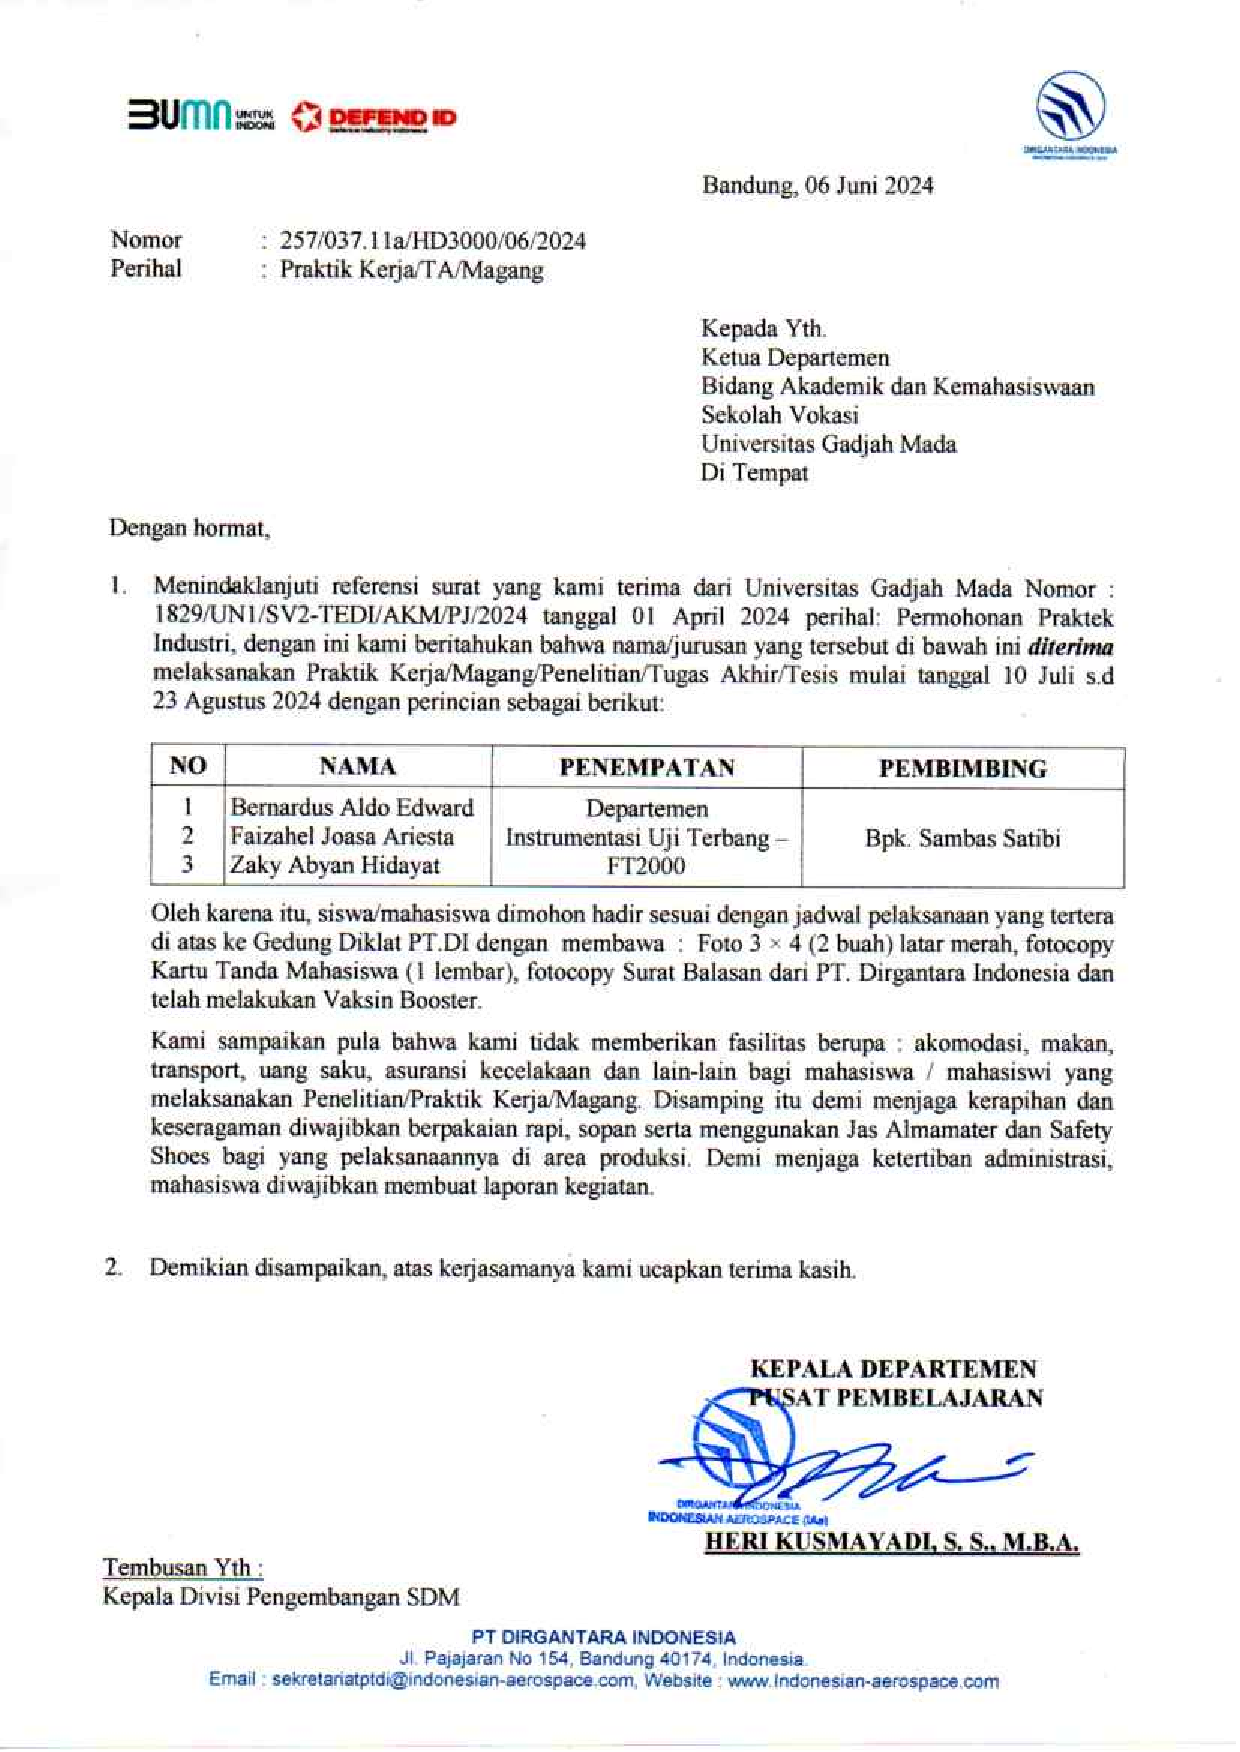
\includegraphics[scale=0.7]{dokumen/magang-ptdi.pdf}

\newpage
\section{Surat Tugas Praktik Industri}
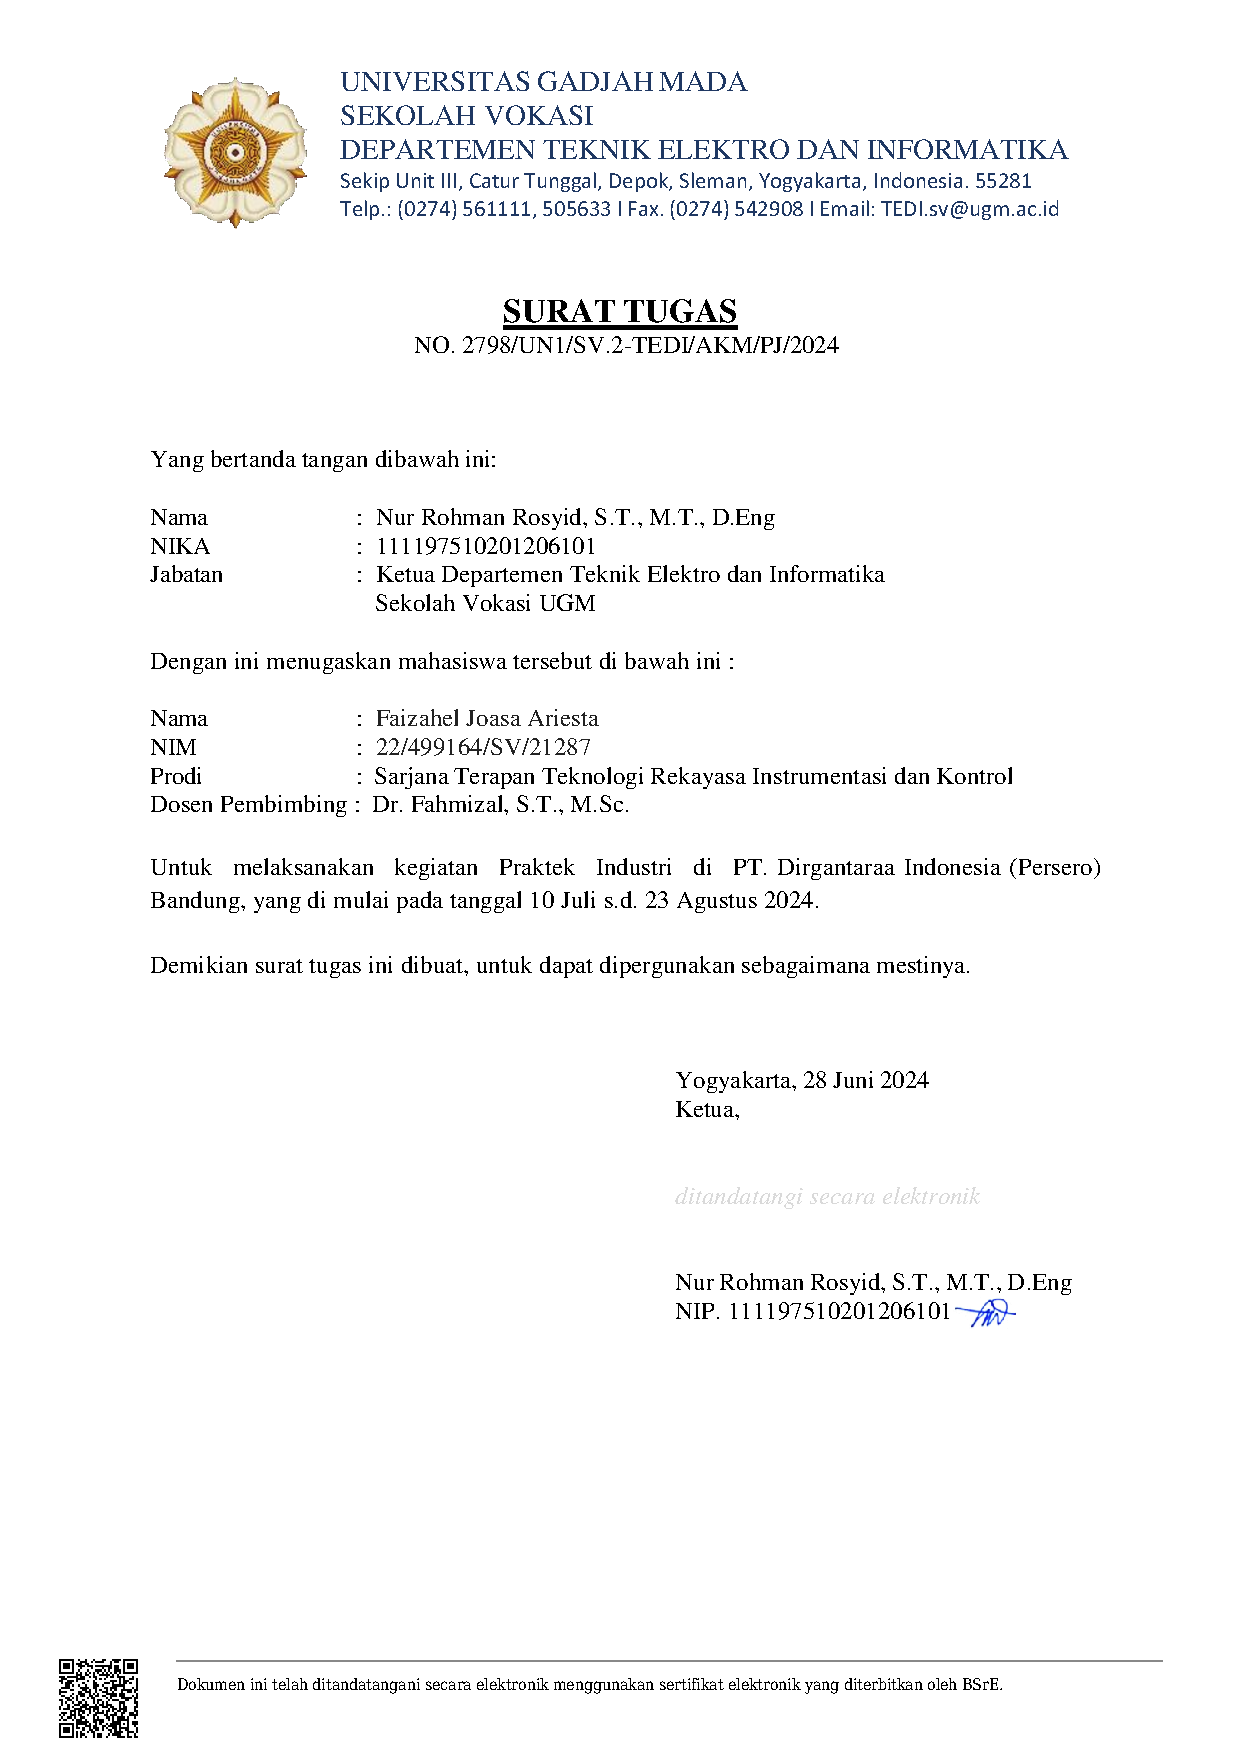
\includegraphics[scale=0.7]{dokumen/suratTugas.pdf}

\newpage
\section{Logbook Kegiatan Praktik Industri}
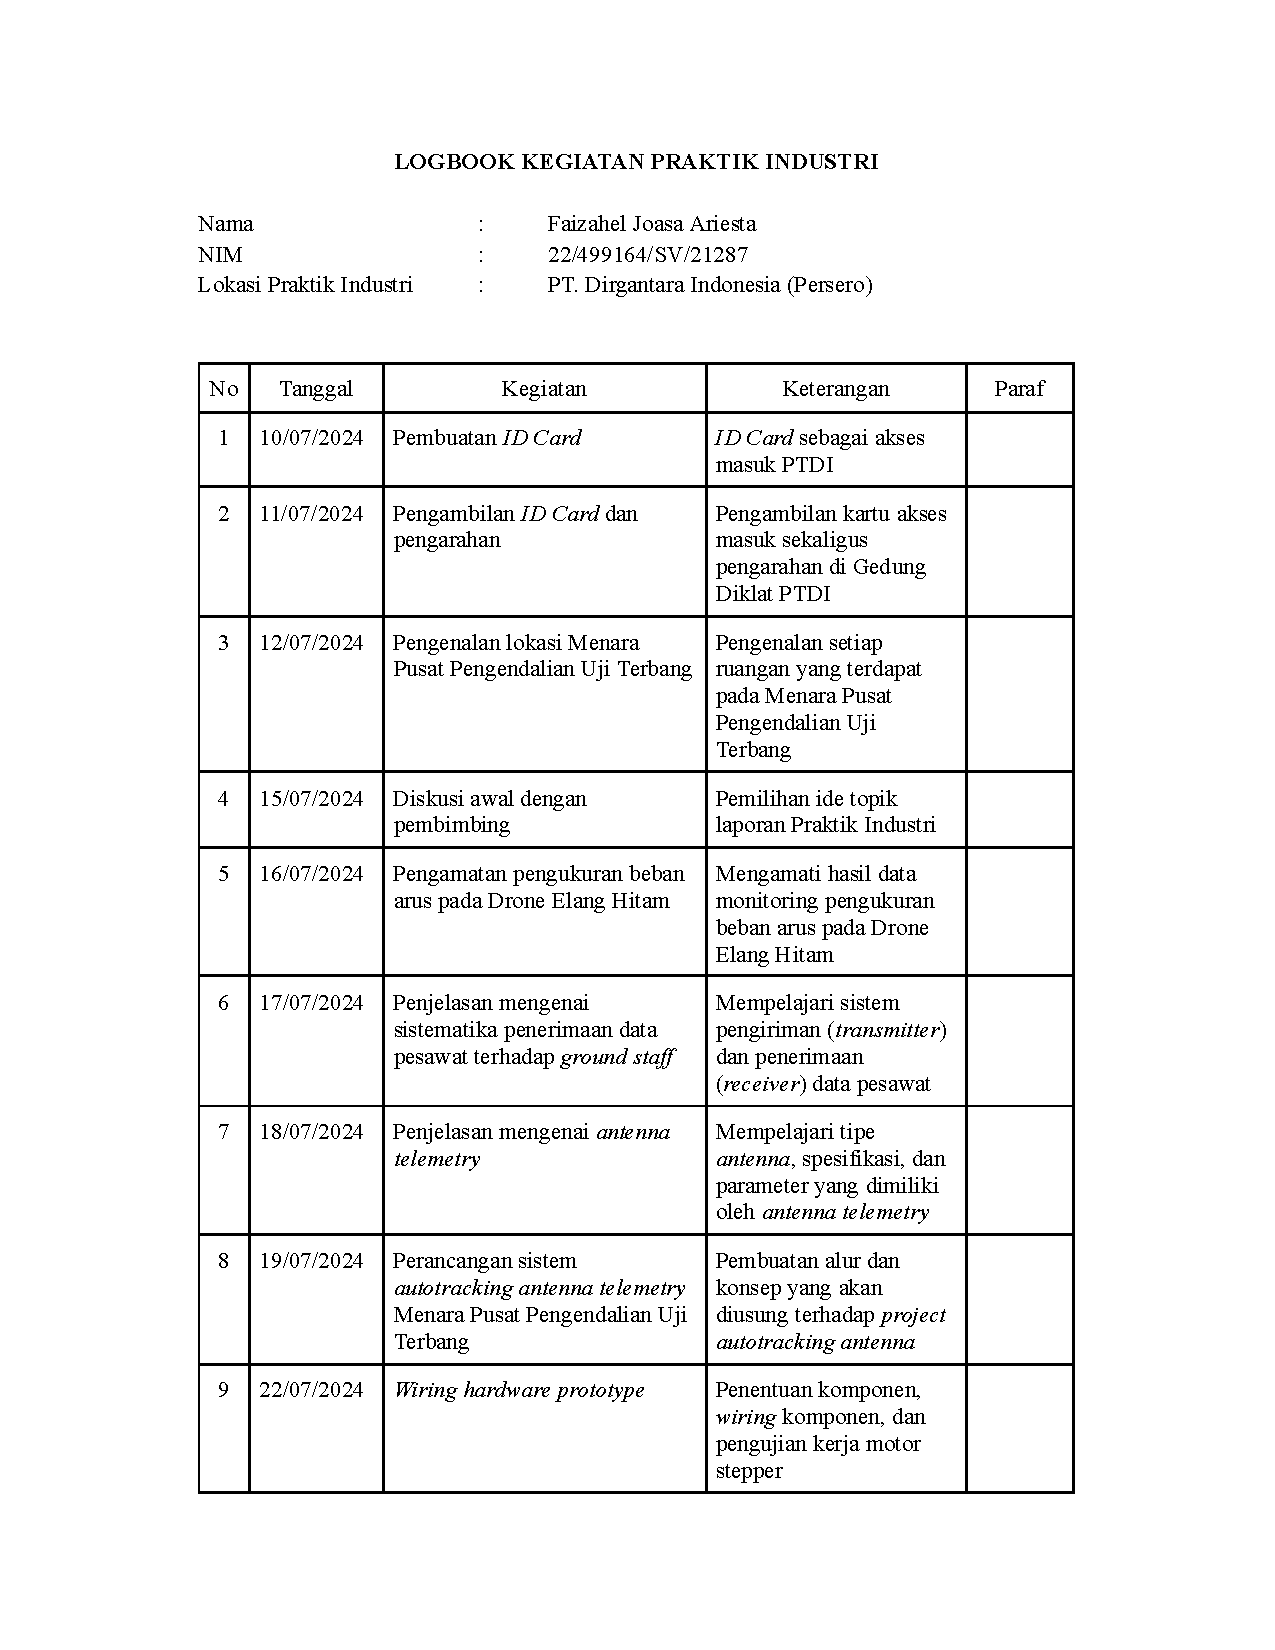
\includegraphics[scale=0.7,page=1]{dokumen/logbook.pdf}
\newpage
\includegraphics[scale=0.7,page=2]{dokumen/logbook.pdf}
\newpage
\includegraphics[scale=0.7,page=3]{dokumen/logbook.pdf}
\newpage
\includegraphics[scale=0.7,page=4]{dokumen/logbook.pdf}

\newpage
\section{Daftar Hadir Praktik Industri}
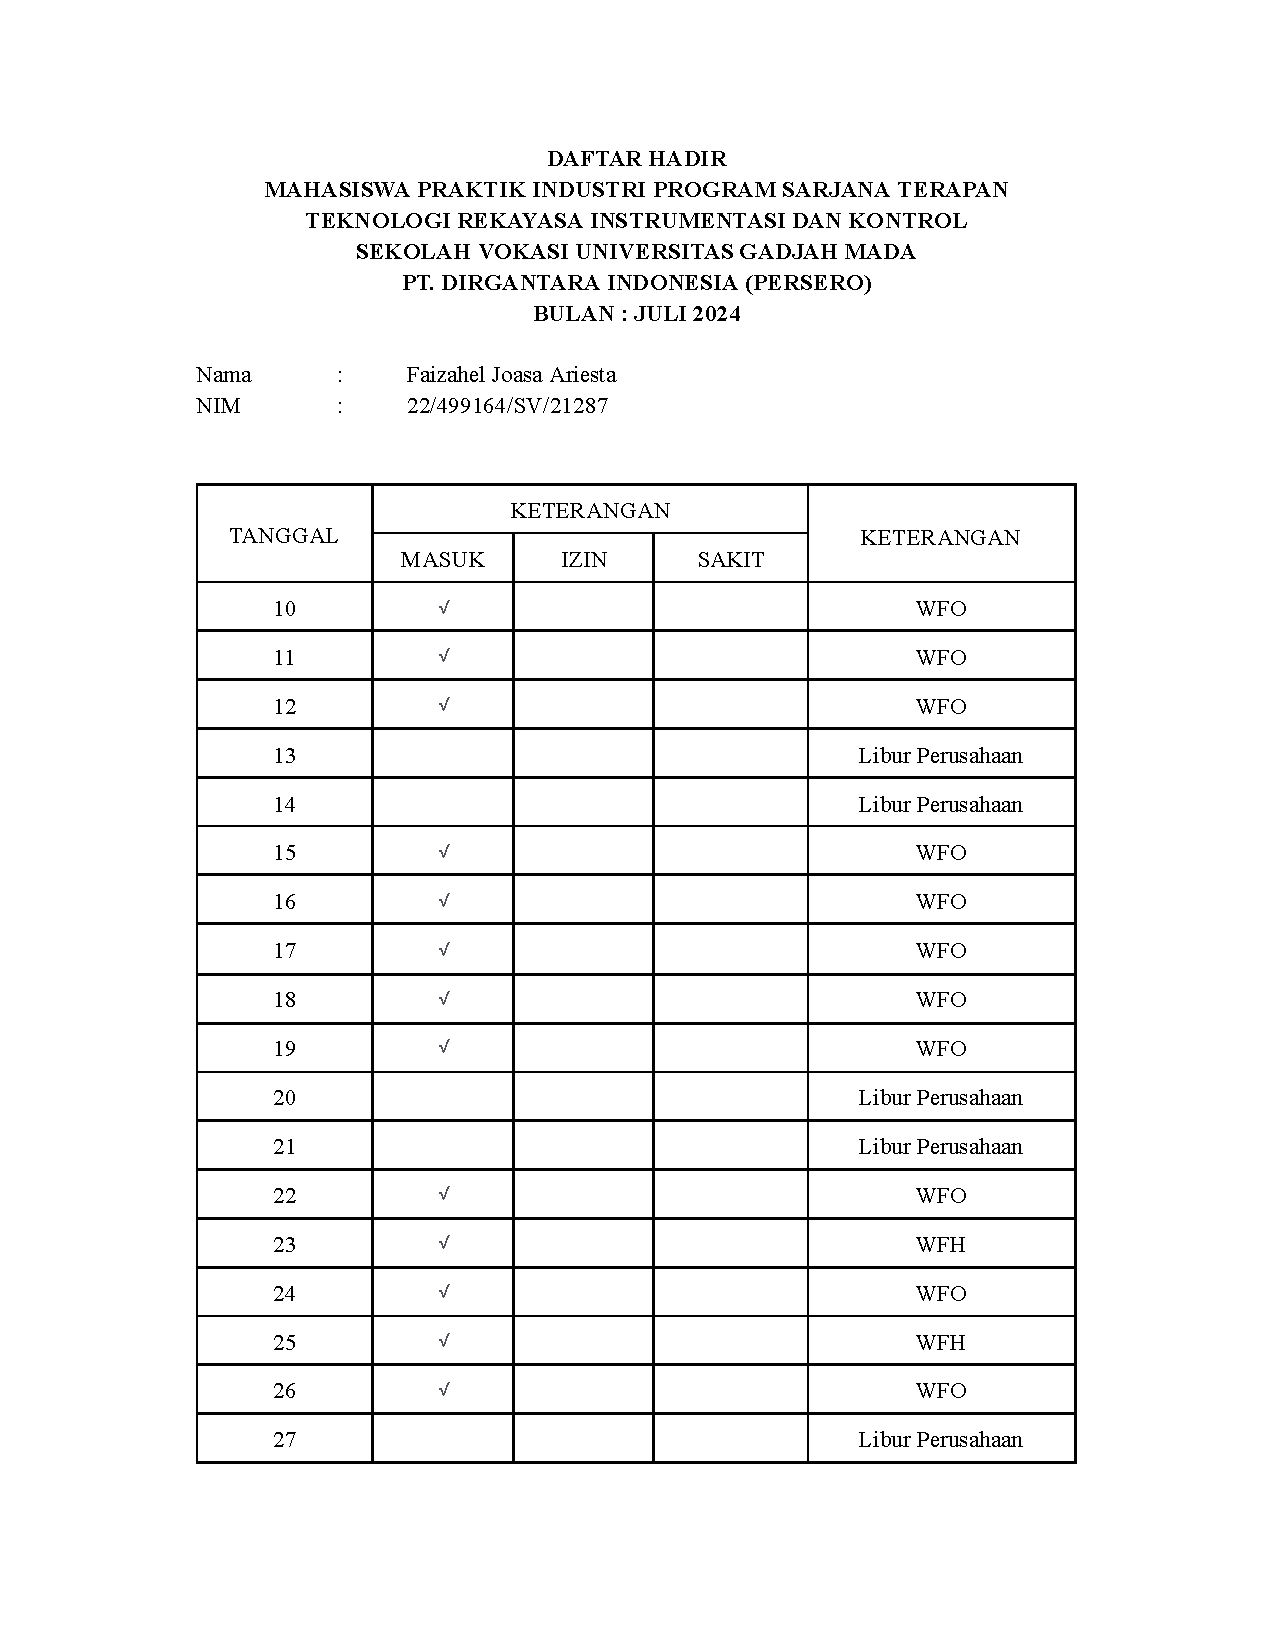
\includegraphics[scale=0.7,page=1]{dokumen/daftarhadir.pdf}
\newpage
\includegraphics[scale=0.7,page=2]{dokumen/daftarhadir.pdf}
\newpage
\includegraphics[scale=0.7,page=3]{dokumen/daftarhadir.pdf}
\newpage
\includegraphics[scale=0.7,page=4]{dokumen/daftarhadir.pdf}


\newpage
\section{Penilaian Hasil Kegiatan Praktik Industri}
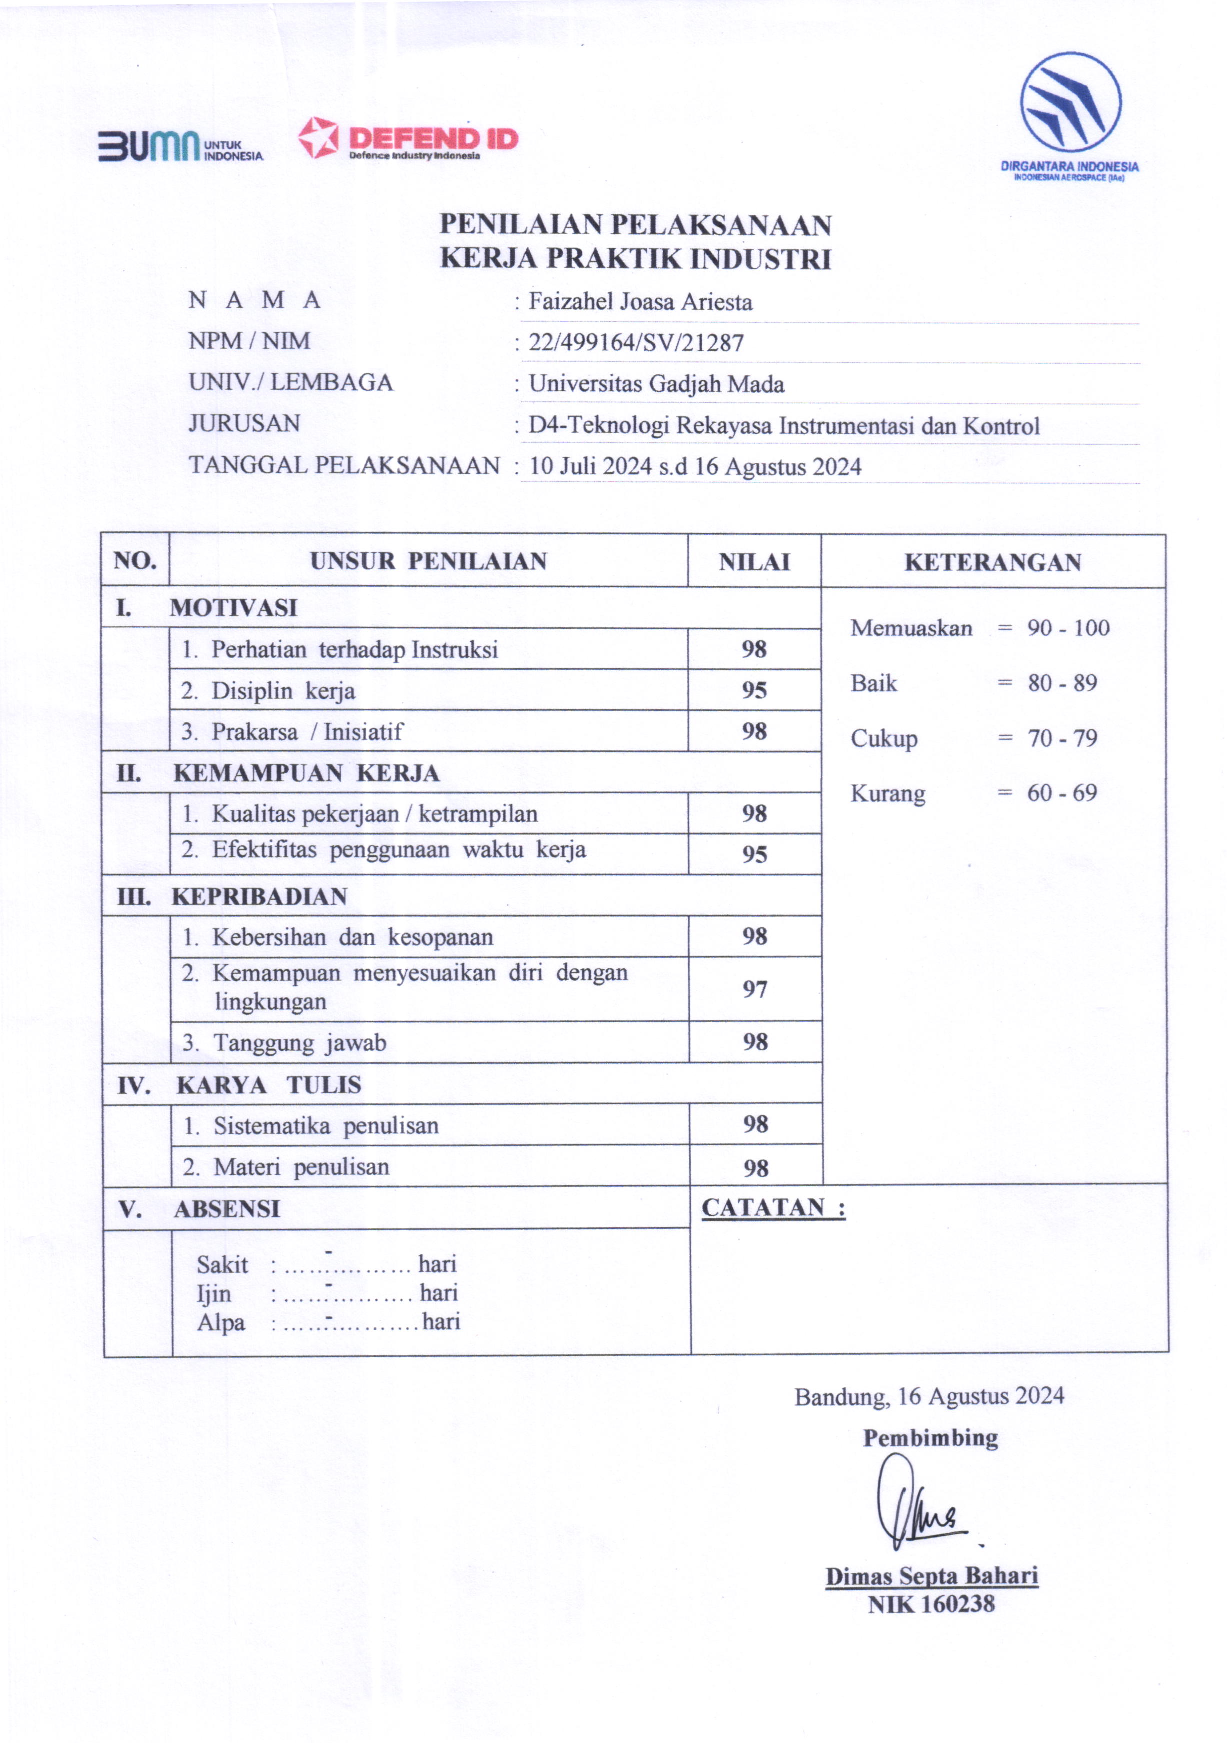
\includegraphics[scale=0.7]{dokumen/nilai-perusahaan.pdf}

\newpage
\section{Surat Keterangan Selesai Praktik Industri}
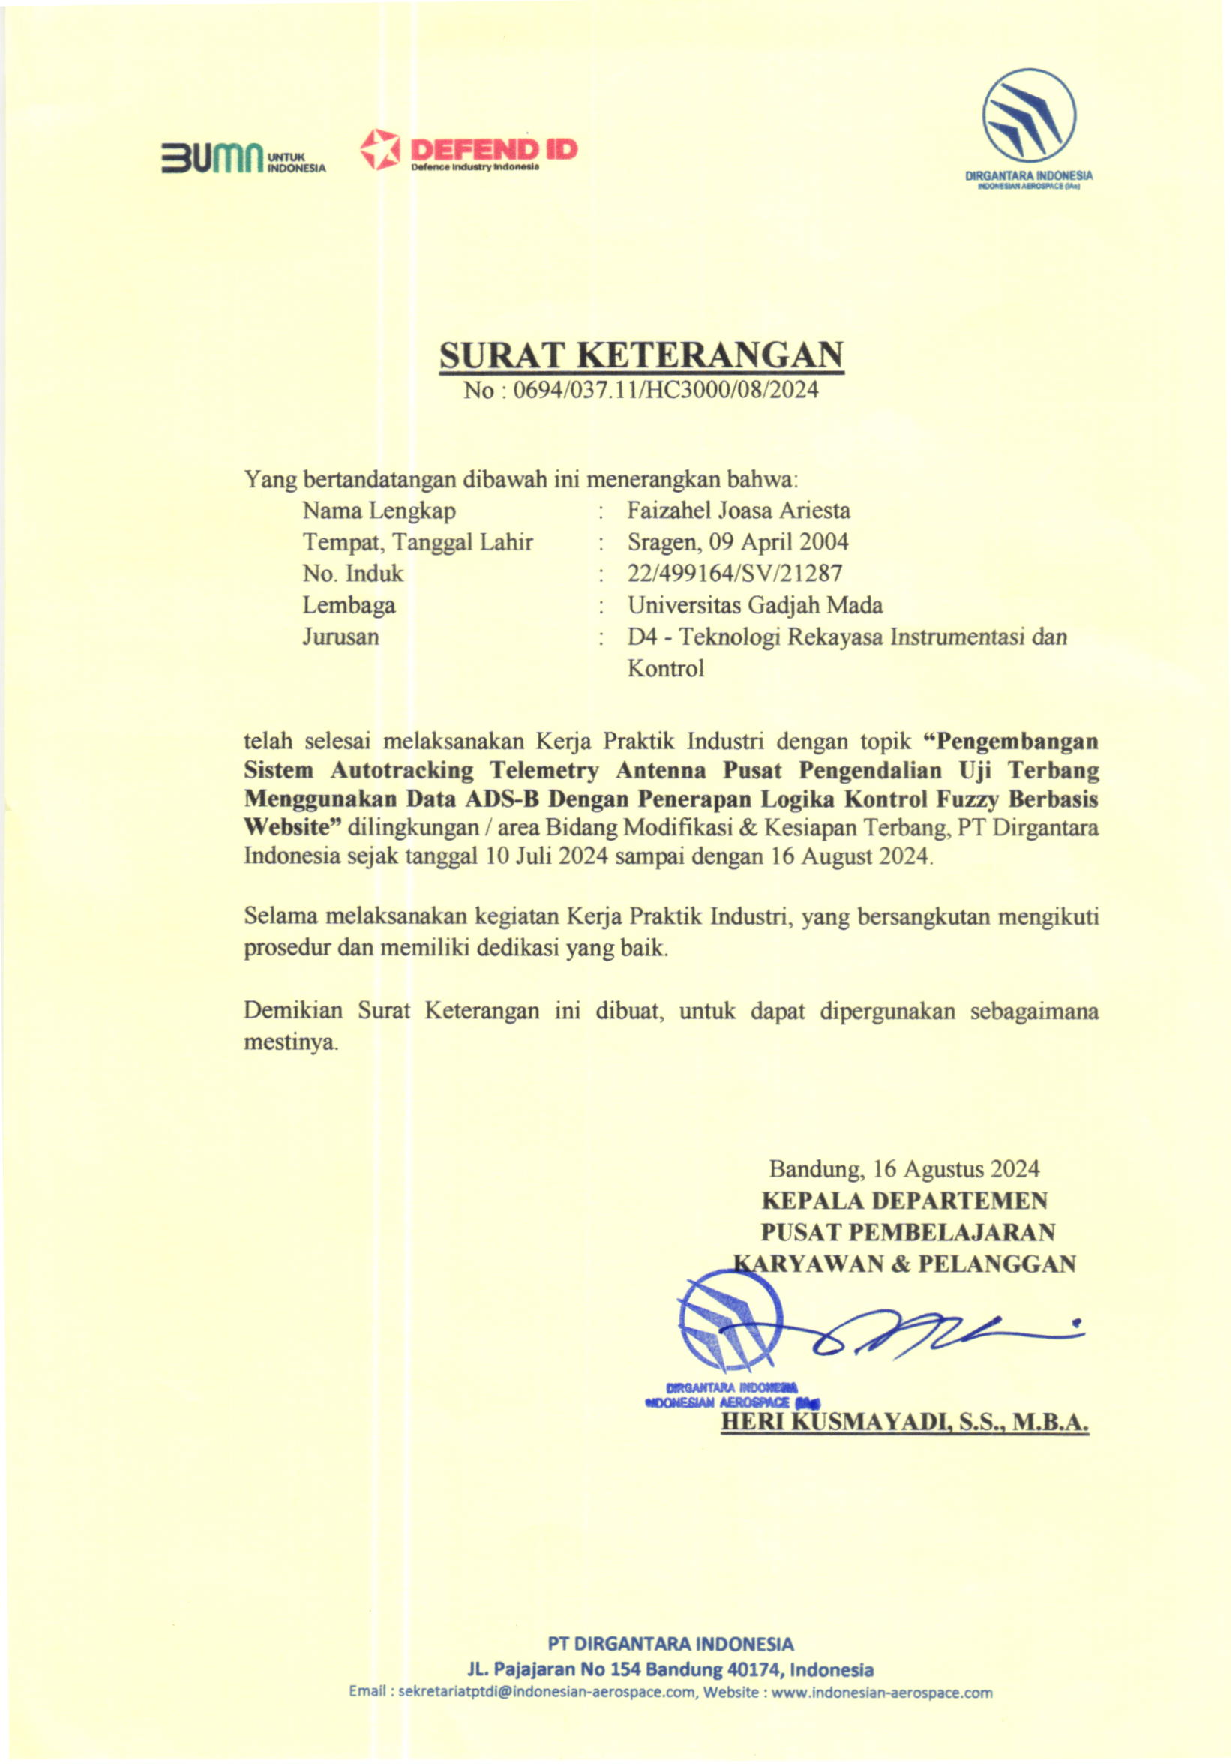
\includegraphics[scale=0.7]{dokumen/pernyataanSelesai.pdf}

\newpage
\section{Dokumentasi}
\begin{figure}[H]
	\centering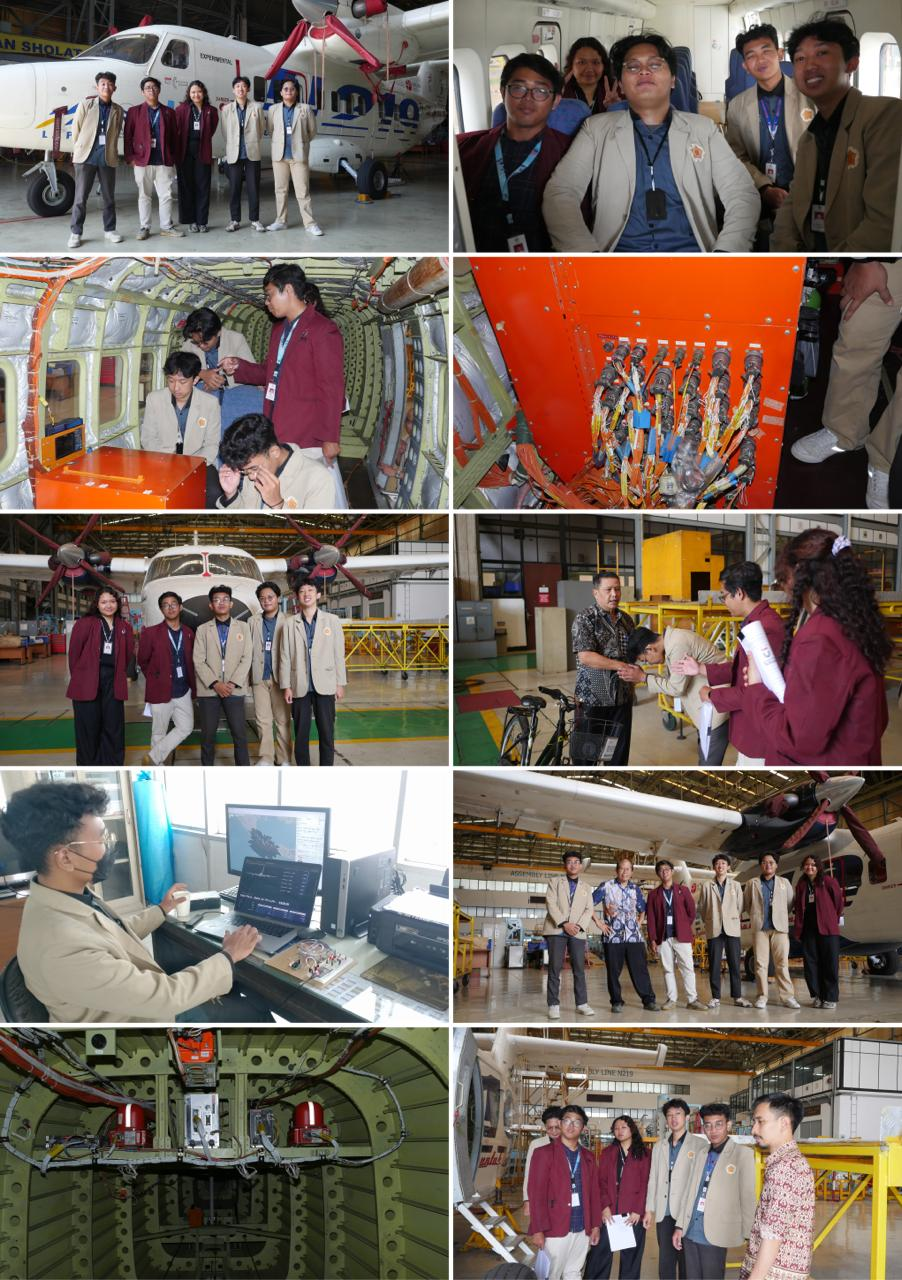
\includegraphics[width = 0.9\textwidth]{gambar/dokumentasi.jpeg}
	\caption{Dokumentasi Kegiatan Praktik Industri di PT Dirgantara Indonesia (Persero)}
\end{figure}





\end{document}

